\chapter{连续介质力学}

在地震学和地球动力学中,我们把地球看作是一个 {\em 连续体\/};
\index{连续体}%
即一个物质的连续分布,物质内部可以有短程与长程的相互作用力。
\index{force!long-range}%
\index{long-range force}%
\index{force!short-range}%
\index{short-range force}%
在本章中,我们对连续介质力学的基本原理做一个简要的回顾,并着重在地球自由振荡及全球地震学现象的研究中最需要的内容。连续介质力学中所研究的数学对象是标量、矢量和张量场;附录~\ref{chapter:vc}简要介绍了我们将会用到的有关多线性代数和多变量微分的一些基本结果。

在从运动学的角度对运动和形变进行讨论之后,我们会概述质量、动量、角动量和能量守恒的基本定律。最低频的地球自由振荡和最长周期的面波受自引力的影响很大;为此我们也会对引力势理论做一个简要的回顾。此外,对这四个守恒定律和牛顿平方反比引力定律的求解还需要引入描述物质物理特性的本构关系。在本章的结尾,我们讨论(非线性)完全弹性体的本构关系。

我们对连续介质力学的讨论虽然很不完整,但与大多的数高等地震学教科书(如\textcite{aki&richards80} 或 \textcite{ben-menahem&singh81}等专著)相比要详尽得多。
特别是在柯西应力之外,我们还引入两种 Piola-Kirchhoff
应力张量,同时,对所有的守恒方程,我们不仅推导出人们较为熟悉的欧拉形式,还推导了拉格朗日形式。
对这些内容的处理我们是以 \textcite{malvern69}为样板,目的是强调其物理含义。
\textcite{marsden&hughes83}采用现代微分几何和泛函分析的语言,在数学上做了更严格的讨论。
有关势函数的理论可以参见 \textcite{kellogg67}的通俗而权威性的专著。

\section{欧拉变量与拉格朗日变量}
\index{Eulerian variable|(}%
\index{Lagrangian variable|(}%

一个连续体的运动有两种可能的表述方式。第一种方式被称为 {\em 拉格朗日\/} 表述,它显然是从对行星围绕太阳旋转这种单个或多个质点运动问题的标准运动学表述推广而来的。
连续体中的质点以其在 $t=0$ 时刻的位置
\index{material particle}%
$\bx$ 来标记,而质点 $\bx$ 在 $t$ 时刻的位置则以 $\br(\bx,t)$表示。
已知所有质点 $\bx$ 在所有 $t \geq 0$ 时刻的位置 $\br(\bx,t)$,则可对物体的运动做完整的运动学表述。
由于 $\bx$ 是质点在
$t=0$ 时刻的位置,因而有 $\br(\bx,0)=\bx$。
运动的时间导数可以用与孤立质点相同的方式来定义;例如,
质点 $\bx$ 在 $t$ 时刻的速度 $\bu^{\rm L}(\bx,t)$ 是 $\bu^{\rm L}=\partial_t\br$。

第二种方式叫做 {\em 欧拉\/}表述,
一个理想化的、遍布各地的气象站可能会用它来报告大气中的气流。所关注的重点不是单个的质点,而是空间中的固定位置(如气象站)。
我们会一贯地用 $\br$ 而非 $\bx$ 来标记空间中的固定位置,而用
$\bu^{\rm E}(\br,t)$ 来表示 $t$ 时刻位于
$\br$ 处的质点的速度。
有了在所有 $t \geq 0$ 时刻连续体占据的所有空间点 $\br$  
的 $\bu^{\rm E}(\br,t$),同样可以对物体的运动做完整的运动学表述。
需要指出的是 $\bu^{\rm E}$ 与
$\bu^{\rm L}$ 是两个不同的场,前者给出的速度是空间位置~$\br$的函数,
而后者则是质点标记 $\bx$ 的函数。为此我们用上角标 $\rm E$ (代表欧拉)
和 $\rm L$ (代表拉格朗日) 来对两者加以区分。

一个运动中的弹性体内任一标量、矢量或张量变量 $q$ 均有其欧拉表述 $q^{\rm E}(\br,t)$ 和拉格朗日表述 $q^{\rm L}(\bx,t)$。
例如,若 $q$ 为温度,则 $q^{\rm E}(\br,t)$
表示的是在空间定点 $\br$ 处所记录的温度,
而 $q^{\rm L}(\bx,t)$ 则表示附着在运动质点 $\bx$上的温度计所记录的温度。这两种表述之间的关系是
\eq
\label{2.ELq}
q^{\rm E}(\br(\bx,t),t)=q^{\rm L}(\bx,t).
\en
这一结果是不言而喻的,因为等式两边所表示的都是在 $t$ 时刻位于 $\br$
处的质点 $\bx$ 所记录的 $q$ 的值。

将等式~(\ref{2.ELq})
对时间求导,利用链式法则我们得到
\eq
\label{2.Ddef}
\partial_tq^{\rm L}=
\partial_tq^{\rm E}+\bu^{\rm E}\cdot\bdel_{\!\subr}q^{\rm E}
\equiv D_tq^{\rm E},
\en
其中 $\bdel_{\!\subr}$ 表示在空间定点 \nolinebreak[2] $\br$ 处的梯度。
\index{gradient!Eulerian}%
\index{Eulerian gradient}%
按~(\ref{2.Ddef}) 式的约定,一个固定在运动质点 $\bx$ 上的观察者会感受到变量 $q$的两种变化:除了空间中静止的观察者所感受到的变化
 $\partial_tq^{\rm E}$ 之外,还有一种因质点在空间梯度
 $\bdel_{\!\subr}q^{\rm E}$ 
中移动而引起的变化 $\bu^{\rm E}\cdot\bdel_{\!\subr}q^{\rm E}$。
我们将这种时间和空间导数的组合
$D_t=\partial_t+\bu^{\rm E}\cdot\bdel_{\!\subr}$
称为 {\em 实质导数\/}
\index{derivative!substantial}%
\index{substantial derivative}%
或 {\em 物质导数}。
\index{material derivative}%
\index{derivative!material}%

在本书的第一部分我们将严格遵循上述符号约定,用上角标 $\rm E$ 和 $\rm L$ 分别表示空间定点 $\br$ 测量到的欧拉变量 $q^{\rm E}$ 和在运动质点 $\bx$ 
上测量到的拉格朗日变量 $q^{\rm L}$。
物质导数 $D_t$ 仅作用在欧拉变量 $q^{\rm E}$ 上,此时 $D_tq^{\rm E}$ 表示在保持 $\bx$ 不变时 $q^{\rm E}(\br(\bx,t),t)$的变化率。通过对相应的拉格朗日变量求一般偏导数 $\partial_tq^{\rm L}$,
也可以得到与运动质点上的观察者所感受到的同样的变化率。
例如,位于 $\br(\bx,t)$
的质点的加速度既可以表示为
$\ba^{\rm L}=\partial_t\bu^{\rm L}=\partial_t^2\br$,也可以写成 $\ba^{\rm E}=D_t\bu^{\rm E}=\partial_t\bu^{\rm E}+\bu^{\rm
E}\cdot\bdel_{\!\subr}\bu^{\rm E}$。

由于一个理想地震仪给出的记录本身是与其相连的质点 $\bx$ 
的运动 $\br(\bx,t)$,地震学使用拉格朗日表述是很自然的。
然而,地震学家们所最熟知的描述应力的柯西应力张量却是欧拉变量。在一般的线性弹性理论中,应力的欧拉本性都被忽略了,这样做的前提是物体内部的初始应力与应力增量具有相同的量级,如大多数工程应用的问题。
然而, \textcite{rayleigh06} 和
\textcite{love11}指出,地球深部的初始应力很大; 正因如此,我们在推导地球的弹性-引力形变所满足的基本定律时必须对应力和其它变量的欧拉与拉格朗日表述认真地做区分。
\index{Eulerian variable|)}%
\index{Lagrangian variable|)}%

\section{形变的度量}
\index{deformation|(}%

要描述形变,我们必须分析空间中邻近两点之间的相对运动,或是追踪两邻近质点的运动。下面我们来讨论欧拉和拉格朗日表述中形变的各种描述以及它们之间的关系。

空间中两邻近点 $\br$ 与 $\br+d\/ \br$ 之间的相对欧拉速度 
$d\/ \bu^{\rm E}$ 是 
$d\/ \bu^{\rm E}=d\/ \br\cdot\bdel_{\!\subr}\bu^{\rm E}$。
我们定义张量 $\bG^{\rm E}$ 
\eq
\bG^{\rm E}=(\bdel_{\!\subr}\bu^{\rm E})^{\rm T},
\en
式中上角标 $\rm T$ 表示转置, $d\/\bu^{\rm E}$
与微分距离 $d\/\br$ 之间的线性关系可以表示成
\eq
d\/ \bu^{\rm E}=\bG^{\rm E}\cdot d\/ \br.
\en
这里的 $\bG^{\rm E}$ 被称为欧拉
{\em 形变率张量\/}。
\index{tensor!deformation-rate}%
\index{deformation-rate tensor}%

如果当前位于 $\br$ 和 $\br+d\/ \br$
的两个质点在初始时分别位于 $\bx$ 和 $\bx+d\/ \bx$,
,那么两质点当前与最初的相对位置矢量
$d\/ \br$ 和 $d\/ \bx$ 有关系
$d\/ \br=d\/ \bx\cdot\bdel_{\!\subx}\br$,
其中 $\bdel_{\!\subx}$ 表示关于质点标记 $\bx$的梯度。
\index{gradient!Lagrangian}%
\index{Lagrangian gradient}%
通过引入如下转置张量 
\eq
\label{2.Fdef}
\bF=(\bdel_{\!\subx}\br)^{\rm T},
\en
我们可以将上述关系写为
\eq
\label{2.drFdx}
d\/ \br=\bF\cdot d\/ \bx.
\en
我们把 $\bF$ 称为 {\em 形变张量}。
\index{tensor!deformation}%
\index{deformation tensor}%
下述条件保证物理上所不允许的现象如弯折、撕裂或反转不会发生
\eq \label{2.detFzero}
{\rm det}\,\bF\not=0,
\en
其中 ${\rm det}\,\bF$ 表示矩阵 $\bF$ 的行列式。

形变率张量 $\bG^{\rm E}$ 和形变张量
$\bF$ 是形变的两个基本度量:
$\bG^{\rm E}(\br,t)$ 给出一个固定点 $\br$ 附近的瞬时形变率,而 $\bF(\bx,t)$ 则是围绕一个移动质点 $\bx$ 的小球体所感受的累积形变。
在数学上更复杂的处理中,
$\bF$ 被认为是一个 {\em 两点张量},
\index{tensor!two-point}%
\index{two-point tensor}%
因为它将当前的变形后相对位置矢量 $d\/ \br$
与初始的变形前相对位置矢量 $d\/ \bx$ 联系起来。
而初始矢量 $d\/ \bx$ 则可借由此两点张量的逆与当前矢量 $d\/ \br$ 联系起来:
\eq
\label{2.Finvrel}
d\/ \bx=\bF^{-1}\cdot d\/ \br.
\en
逆张量 $\bF^{-1}$ 满足 $\bF\cdot\bF^{-1}=\bF^{-1}\cdot\bF=\bI$,
这里 $\bI$ 是单位张量。 (\ref{2.detFzero}) 的限制条件保证了 $\bF^{-1}$ 的存在。严格来说,应该有两个单位张量 $\bI$,
一个在变形前的形态中,另一个在变形后的形态中;
不过,在此后的讨论中我们将忽略这些由 $\bF$ 与 $\bF^{-1}$ 的两点特性所引起的细微差异。

$\bG^{\rm E}$ 和 $\bF$ 这两个张量之间存在着关系
\eq
\label{2.FrelG}
\partial_t\bF=\bG^{\rm E}\cdot\bF,
\en
或者可等效地表示为
\eq
\label{2.FrelG2}
\bG^{\rm E}=\partial_t\bF\cdot\bF^{-1}.
\en
可通过将定义式~(\ref{2.Fdef})对时间求导,然后使用链式法则来证明等式~(\ref{2.FrelG}) 。

我们可以将形变率张量 $\bG^{\rm E}$
表示为一个对称张量和一个反对称张量的和:
\eq
\label{2.GDW}
\bG^{\rm E}=\bD^{\rm E}+\bW^{\rm E},
\en
其中
\eq
\bD^{\rm E}=\half[\bG^{\rm E}+(\bG^{\rm E})^{\rm T}],\qquad
\bW^{\rm E}=\half[\bG^{\rm E}-(\bG^{\rm E})^{\rm T}].
\en
式中对称部分 $\bD^{\rm E}=(\bD^{\rm E})^{\rm T}$
是欧拉 {\em 是欧拉应变率张量\/},
\index{tensor!strain-rate}%
\index{strain-rate tensor}%
而反对称部分 $\bW^{\rm E}=-(\bW^{\rm E})^{\rm T}$
则是转动率或 {\em 涡度张量}。
\index{tensor!vorticity}%
\index{vorticity tensor}%
\index{tensor!rotation-rate}%
\index{rotation-rate tensor}%
利用等式~(\ref{2.GDW}) 我们可以将微分速度矢量 $d\/ \bu^{\rm E}$ 
分解为分别与局地应变率和局地转动率相对应的两个部分:
\eq
d\/ \bu^{\rm E}=\bD^{\rm E}\cdot d\/ \br+\bW^{\rm E}\cdot d\/ \br.
\en
欧拉速度的旋度,即涡度矢量
$\bdel_{\!\subr}\times\bu^{\rm E}$,
与涡度张量 $\bW^{\rm E}$ 之间有如下关系
\eq
\bdel_{\!\subr}\times\bu^{\rm E}=-\wedge\hspace{-0.5 mm}\bW^{\rm E},
\en
其中 $\wedge$ 表示楔形算子,
\index{operator!wedge}%
\index{wedge operator}%
其定义请见附录~A.1.6.
欧拉速度微分 $d\/ \bu^{\rm E}$
中与 $\bW^{\rm E}$ 相关的部分可以用 $\bdel_{\!\subr}\times\bu^{\rm E}$ 表示成如下形式:
\eq
\bW^{\rm E}\cdot d\/ \br=\half(\bdel_{\!\subr}\times\bu^{\rm E})\times d\/ \br.
\en
上述关系表明了将 $\bW^{\rm E}$ 称为
``涡度张量''
的合理性,同时也表明 
$\bdel_{\!\subr}\times\bu^{\rm E}$ 是 
$t$ 时刻在 $\br$ 处周围物质的瞬时角速度的两倍。
至于将 $\bD^{\rm E}$ 称为
``应变率张量'' 的合理性,我们可以考虑微分长度平方
$\|d\/ \br\|^2$的变化率,
通过简单的推导可以得到如下关系:
\eqa
\lefteqn{
{d\over dt}\| d\/ \br \|^2\,=
2(d\/ \br\cdot\partial_t\bF\cdot d\/\bx)} \nonumber \\
&&\mbox{}\qquad\!\!=2(d\/ \br\cdot\partial_t\bF\cdot\bF^{-1}\cdot d\/ \br)=
2(d\/ \br\cdot\bG^{\rm E}\cdot d\/ \br),
\ena
这里我们使用了式~(\ref{2.drFdx}),
(\ref{2.Finvrel})~和~(\ref{2.FrelG2})。
因为涡度张量 $\bW^{\rm E}$ 是反对称的,它对二次型乘积
$d\/ \br\cdot\bG^{\rm E}\cdot d\/ \br$ 没有贡献;
因而相对位置矢量长度的平方 $\| d\/ \br \|^2$
的变化率可以由应变率完全确定:
\eq \label{2.Lyme}
{d\over dt}\| d\/ \br\|^2\,=2(d\/ \br\cdot\bD^{\rm E}\cdot d\/ \br).
\en

拉格朗日 {\em 应变张量\/}
\index{tensor!strain}%
\index{strain tensor}%
$\bE^{\rm L}$ 是通过初始和当前的长度平方 $\| d\/ \bx\|^2$ 和 $\| d\/ \br\|^2$
定义的
\eq
\label{2.Edef}
\| d\/ \br\|^2-\| d\/ \bx\|^2\,=
2(d\/ \bx\cdot\bE^{\rm L}\cdot d\/ \bx).
\en
考虑到
\eq
\label{2.drsq}
\| d\/ \br\|^2\,=(\bF\cdot d\/ \bx)\cdot
(\bF\cdot d\/ \bx)=d\/\bx\cdot
(\bF^{\rm T}\cdot\bF)\cdot d\/ \bx.
\en
我们可以在 $\bE^{\rm L}$ 与形变张量 $\bF$ 
之间建立如下关系
\eq
\label{2.EFrel}
\bE^{\rm L}=\half(\bF^{\rm T}\cdot\bF-\bI).
\en
张量 $\bE^{\rm L}$ 给出的是从 $t=0$ 
时刻开始在质点 $\bx$
附近的物质所累积的总的有限应变。
从式~(\ref{2.EFrel})
可以清楚看到这一累积应变是对称的,即 $(\bE^{\rm L})^{\rm T}=\bE^{\rm L}$.

随质点 $\bx$ 运动的观察者所感受到的瞬时应变率是
$\partial_t\bE^{\rm L}$。
要想得到这个拉格朗日应变率与欧拉应变率
$\bD^{\rm E}$ 之间的关系,我们考虑如下等式
\eq
\label{2.drdx1}
{d\over dt}\left(\|d\/ \br\|^2-\| d\/ \bx\|^2\right)=
2(d\/\bx\cdot\partial_t\bE^{\rm L}\cdot d\/ \bx).
\en
然而,因为 $d\/\bx$ 是不变的,于是我们有
\eq
\label{2.drdx2}
{d\over dt}\!\left(\|d\/ \br\|^2-\| d\/ \bx\|^2\right)=
{d\over dt}\|d\/ \br\|^2\,=
2[d\/ \bx\cdot(\bF^{\rm T}\cdot\bD^{\rm E}\cdot\bF)\cdot d\/ \bx],
\en
这里使用了式~(\ref{2.drFdx})~和~(\ref{2.Lyme})。
通过比较式~(\ref{2.drdx1})
和~(\ref{2.drdx2}) 中的结果,我们发现
\eq
\partial_t\bE^{\rm L}=\bF^{\rm T}\cdot\bD^{\rm E}\cdot\bF,
\en
或者等效于
\eq
\label{2.DEdtEL}
\bD^{\rm E}=\bF^{-\rm T}\cdot\partial_t\bE^{\rm L}\cdot\bF^{-1}.
\en

\begin{figure}[!b]
\begin{center}
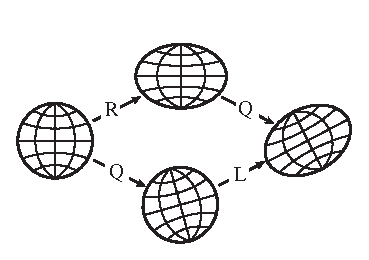
\includegraphics{../figures/chap02/fig01.eps}
\end{center}
\caption[poldecomp]{\label{fig2.1}
形变张量的球极分解 ${\bf F}={\bf Q}\cdot{\bf R}={\bf L}\cdot{\bf Q}$的示意图。围绕质点
$\bf x$ 的一个无穷小球体可以先做伸展 $\bf R$ 而后做转动 $\bf Q$ ({\em 上}) 或者先做转动 $\bf Q$ 而后做伸展 $\bf L$ ({\em 下})。}
\end{figure}
根据 {\em 球极分解定理},
\index{polar decomposition}%
形变张量 $\bF$ 可以用唯一的方式表示成如下两种形式之一
\eq
\label{2.poldecomp}
\bF=\bQ\cdot\bR=\bL\cdot\bQ.
\en
分解式~(\ref{2.poldecomp})中的两个张量 $\bR$ 和 $\bL$ 均为对称的正定张量:
\eq
\bR^{\rm T}=\bR,\qquad\bL^{\rm T}=\bL,
\en
而 $\bQ$ 则是一个正交张量:
\eq
\bQ^{\rm T}\cdot\bQ=\bQ\cdot\bQ^{\rm T}=\bI.
\en
我们称对称张量 $\bR$ 和 $\bL$ 分别为
{\em 右伸展\/} 和 {\em 左伸展张量\/},
\index{tensor!right stretch}%
\index{tensor!left stretch}%
\index{stretch tensor!right}%
\index{stretch tensor!left}%
称正交张量 $\bQ$ 为
{\em 转动张量}。
\index{tensor!rotation}% 
\index{rotation tensor}% 
伸展张量可以用
$\bF$ 以显式表示为
\eq
\label{2.RFrel}
\bR=(\bF^{\rm T}\cdot\bF)^{1/2},\qquad
\bL=(\bF\cdot\bF^{\rm T})^{1/2}.
\en
右伸展张量 $\bR$ 与应变张量 $\bE^{\rm L}$
密切相连;通过比较式~(\ref{2.EFrel})~和~(\ref{2.RFrel})
我们看到
\eq
\label{2.RErel}
\bR=(\bI+2\bE^{\rm L})^{1/2}.
\en
式~(\ref{2.poldecomp}) 对球极分解的物理解释是很清楚的:围绕质点
$\bx$ 的一个无穷小球体的形变既可以被看作是先经过对称伸展 $\bR$ 而后做刚体转动 $\bQ$,
也可以被看作是先经过有限动转 $\bQ$ 而后做对称伸展 $\bL$ (见图~\ref{fig2.1})。
两个伸展张量互为转动的结果,即两者之间可以用正交变换相连: $\bR=\bQ^{\rm T}\cdot\bL\cdot\bQ$.
\index{deformation|)}%

\section{体积与面积变化}
\index{volume change|(}%
\index{area change|(}%

在结束对运动学的回顾之前,我们来讨论一下无穷小连续体内体积元与面积元所遵循的变换公式。
我们先来考虑一个在$t=0$ 时刻围绕质点 $\bx$ 的体积为
$dV^0$ 的无穷小球体,在后续时刻 $t$,小球体移动到了 $\br$ 处,并且经历了转动与变形;我们将其新的体积用 $dV^t$ 表示。我们可以计算这个无穷小体积元在变形后与变形前的体积比
\eq
\label{2.Jdef}
J={dV^t \over dV^0},
\en
因为这个比值无非就是从质点 $\bx$ 坐标系到空间 $\br$ 
坐标系变换的雅可比
\index{Jacobian!of transformation}%
\index{transformation!Jacobian of}%
\eq
J=\det\bF。
\en

我们接下来考虑一个在变形前的形态中以质点 $\bx$ 
为中心的带方向的无穷小表面面积元
$\bnh^0 d\/ \Sigma^0$。
在 $t$ 时刻,该面积元已经移动到 $\br$ 处并且经历了转动与伸展而成为 $\bnh^t d\/ \Sigma^t$。
我们试图建立变形前的面积元 $\bnh^0 d\/ \Sigma^0$ 与变形后的面积元 $\bnh^t d\/ \Sigma^t$ 之间的关系。
为简化计算,我们考虑变形前后的两个无穷小平行四边形,其边长分别为 $d\/ \bx$ \times $\delta \bx$ 
和 $d\/ \br$ \times $\delta \br$ (见图~2.2)。
\begin{figure}[!b]
\centering
\begin{tabular}{lr}
\begin{tabular}{l}
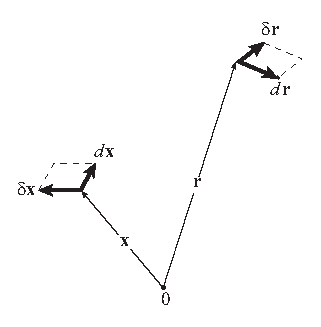
\includegraphics{../figures/chap02/fig02.eps}
\end{tabular}
&
\parbox{4.0cm}{\small
图~2.2. 在变形前的初始时刻位于 ${\bf x}$ 点的平行四边形
$\hat{\bf n}^0 d\/ \Sigma^0 = d\/{\bf x} \times \delta{\bf x}$ 在 $t$ 时刻成为位于 ${\bf r}$ 处的变形后的平行四边形
$\hat{\bf n}^t d\/ \Sigma^t = d\/{\bf r}
\times \delta{\bf r}$。
两个无穷小的面积元之间的关系为式~(\ref{2.ndsigrel}).}
\end{tabular}
\end{figure}
\addtocounter{figure}{1}
$\bnh^0 d\/ \Sigma^0$ 和 $\bnh^t d\/ \Sigma^t$
这两个量可以分别表示为
\eq
\label{2.ndsig}
\bnh^0 d\/ \Sigma^0 = d\/ \bx \times \delta \bx, \qquad
\bnh^t d\/ \Sigma^t = d\/ \br \times \delta \br.
\en
引入笛卡尔坐标系 $\bxh_1$, $\bxh_2$, $\bxh_3$,
我们可以把式~(\ref{2.ndsig}) 写成分量形式
\eq
\label{2.ndsig3}
n_i^0 d\/ \Sigma^0 = \ep_{ijk} \,d\/ x_j \,\delta x_k, \qquad
n_l^t d\/ \Sigma^t = \ep_{lmn} \,d\/ r_m \,\delta r_n.
\en
将 $d\/ x_j = F_{jm}^{-1} d\/ r_m$ 和
$\delta x_k = F_{kn}^{-1} \delta r_n$
带入~(\ref{2.ndsig3}) 中的第一个等式,我们得到
\eq
\label{2.ndsig5}
n_i^0 d\/ \Sigma^0 = \ep_{ijk}\,F_{jm}^{-1}
F_{kn}^{-1}\,d\/ r_m \,\delta r_n.
\en
在~(\ref{2.ndsig5}) 的两边同时乘以
$F_{il}^{-1}$ 并利用下面的等式
\eq
J^{-1}\ep_{lmn} = \ep_{ijk}\,F_{il}^{-1}F_{jm}^{-1}F_{kn}^{-1}
\en
则可以得到
\eq
\label{2.ndsig6}
F_{il}^{-1}n_i^0 d\/ \Sigma^0 = J^{-1} \ep_{lmn} \,d\/ r_m \,\delta r_n
= J^{-1} n_l^t d\/ \Sigma^t,
\en
其中最后一个等号需要利用~(\ref{2.ndsig3})中的第二个等式。
转回到与坐标系无关的矢量形式,
~(\ref{2.ndsig6}) 可以最终表示成
\eq
\label{2.ndsigrel}
\bnh^t d\/ \Sigma^t = J \, \bnh^0  d\/ \Sigma^0 \cdot \bF^{-1}.
\en
这一联系 $\bnh^t d\/ \Sigma^t$ 与
$\bnh^0 d\/ \Sigma^0$ 
的关系式是体积关系式 $d\/ V^t = J\, d\/ V^0$ 的面积形式。
\index{volume change|)}%
\index{area change|)}%

\section{雷诺兹输运定理}
\index{Reynolds transport theorem|(}%
\index{transport theorem|(}%

令 $V^t$ 为随物体移动的任意体积,其内部及边界 $\p V^t$ 始终由同样的质点组成, 如图~\ref{fig2.3} 所示。
假设 $q^{\rm E}$ 是遍布于连续体内的力学或热力学量的体密度,我们来考虑在
$V^t$ 内部这个总的 ``q量'' 随时间
$t$ 的变化率。
\index{q-stuff}%
被积函数 $q^{\rm E}$ 和积分区域 $V^t$
均随时间 $t$ 变化;因此在
{\em 同步移动\/} 的体积 $V^t$ 内的积分对时间的全导数是
\index{co-moving volume}%
\index{volume!co-moving}%
\eq
\label{2.dtint}
{d\over dt} \int_{V^t} q^{\rm E} \,dV^t =
\int_{V^t} \partial_t q^{\rm E} \,dV^t +
\int_{\partial V^t} (\bnh^t \cdot \bu^{\rm E}) q^{\rm E} \,d\/\Sigma^t,
\en
其中 $\bnh^t$ 是 $\p V^t$ 上向外的单位法向矢量,
这里我们用上角标 $t$ 来提醒我们微分体积元 $dV^t$ 和面积元 $d\/\Sigma^t$
是同步移动的。
等式~(\ref{2.dtint}) 中第一项是由局地的密度空间变化 $\partial_tq^{\rm E}$引起的, 而第二项则代表由流过移动中边界的通量 
$(\bnh^t\cdot\bu^{\rm E})q^{\rm E}$ 所带来的变化。
将高斯定理应用于 $\p V^t$ 上的表面积分,我们有
\eq
\label{2.reynolds}
{d\over dt} \int_{V^t} q^{\rm E} \,dV^t =
\int_{V^t}[\partial_t q^{\rm E} + \bdel_{\!\subr}
\cdot (\bu^{\rm E}q^{\rm E})]\, dV^t.
\en
\begin{figure}
\begin{center}
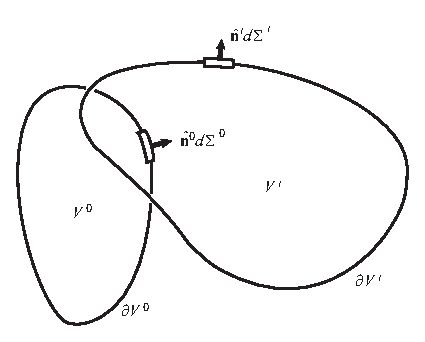
\includegraphics{../figures/chap02/fig03.eps}
\end{center}
\caption[comoving]{\label{fig2.3}
欧拉形式的守恒定律是通过考虑一个移动中的体积得到的,该体积内部的物质组成始终不变。组成初始体积 $V^0$ 的边界 $\partial V^0$ 上的面积元
$\hat{\bf n}^0d\/ \Sigma^0$ 
的质点移动到变形后体积 $V^t$ 的边界 $\partial V^t$ 上的面积元 $\hat{\bf n}^t  d\/ \Sigma^t$。}
\end{figure}
这一结果称为 {\em 雷诺兹输运定理},
它将移动中体积内积分的时间导数表示为在同一体积内的积分。
式~(\ref{2.reynolds}) 中的 $q^{\rm E}$ 可以是标量、矢量或是张量;需要记住的是,如果 $q^{\rm E}$ 不是标量,那么张量乘积是不可交换的,即: $\bu^{\rm E}q^{\rm E} \not= q^{\rm E}\bu^{\rm E}$。
我们将在第~\ref{2.sec.euleq} 节中利用雷诺兹输运定理,
以任意移动中的体积内积分形式的平衡原理,推导出欧拉形式的质量、动量、角动量和能量守恒定律。
\index{transport theorem|)}%
\index{Reynolds transport theorem|)}%

\section{应力的度量}
\index{stress!measures of|(}%
\index{tensor!stress|(}%
\index{stress tensor|(}%

\begin{figure}[!t]
\centering
\begin{tabular}{lr}
\begin{tabular}{l}
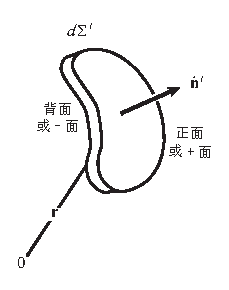
\includegraphics{../figures/chap02/fig04.eps}
\end{tabular}
&
\parbox{5.5cm}{\small
图~2.4. 带有方向的表面面积元 $\hat{\bf n}^t  d\/ \Sigma^t$ 的正面 $+$
和背面 $-$。 本书中我们将一贯遵循这一符号规则。}
\end{tabular}
\end{figure}
\addtocounter{figure}{1}
\index{force!short-range}%
\index{short-range force}%
连续介质力学中分子之间的短程作用力是用 {\em 应力张量}来表示的。
应力可以用三种不同的方法来度量或定义,每一种定义在地球的弹性-引力形变的理论中有各自的作用。最为人们熟知的度量是 {\em 柯西应力\/},
\index{stress!Cauchy}%
\index{Cauchy stress}%
它的定义方式如下。
令 $\bnh^t d\/ \Sigma^t$ 
为一个在 $t$ 时刻以固定点 $\br$ 为中心的带有方向的表面面积元;
我们称法向矢量 $\bnh^t$ 所指向的一侧为面积元的正面或 $+$ 面,
而称另外一侧为背面或 $-$ 面 (见~图~2.4).
若以 $d\/ \bef^{\rm E}$ 表示紧贴面积元正面的所有质点作用在紧贴背面的所有质点的瞬时面力,
这个透过面元的作用力 $d\/ \bef^{\rm E}$ 可以用欧拉柯西应力 
$\bT^{\rm E}$
表示成如下形式:
\eq
\label{2.TEdef}
d\/ \bef^{\rm E} = \bnh^t d\/ \Sigma^t \cdot \bT^{\rm E}.
\en
与任何其它变量一样,柯西应力也有拉格朗日和欧拉表述;
相应的拉格朗日应力
$\bT^{\rm L}$ 的定义同样是
$\bT^{\rm L}(\bx,t)=\bT^{\rm E}(\br(\bx,t),t)$。
欧拉应力 $\bT^{\rm E}$ 很自然地出现在欧拉形式的动量守恒定律中,而相应的拉格朗日形式的守恒定律则不能很容易地以 $\bT^{\rm L}$ 来表示。

能够使拉格朗日动量方程的形式最为简单的应力度量是所谓的 {\em 第一类 Piola-Kirchhoff 应力}.
\index{stress!first Piola-Kirchhoff}%
\index{Piola-Kirchhoff stress!first}%
这个以
$\bT^{\rm PK}$ 表示的量的定义是
\eq
\label{2.TPKdef}
d\/ \bef^{\rm E} = \bnh^0 d\/ \Sigma^0 \cdot \bT^{\rm PK}.
\en
很明显, $\bT^{\rm PK}$ 将作用在位于 $\br$ 处的变形后面积元 
$\bnh^td\/\Sigma^t$ 上的力 $d\/ \bef^{\rm E}$
用位于初始位置 $\bx$ 处变形前的面积元 
$\bnh^0d\/\Sigma^0$ 来表示。
此外,第一类
Piola-Kirchhoff 应力 $\bT^{\rm PK}$ 表示的是变形前单位面积上的力,
而欧拉柯西应力 $\bT^{\rm E}$ 与拉格朗日柯西应力 $\bT^{\rm L}$ 均为变形后单位面积上的力。
我们可以用变形前后面积元之间的变换式 (\ref{2.ndsigrel}) 得到$\bT^{\rm PK}$ 和 $\bT^{\rm L}$
之间的关系;结果可以表示成两个等价的形式
\eq
\label{2.tpkt1}
\bT^{\rm PK}=J\,\bF^{-1}\cdot\bT^{\rm L},\qquad
\bT^{\rm L}=J^{-1}\bF\cdot\bT^{\rm PK}.
\en
式 (\ref{2.TPKdef}) 中的表面力 $d\/\bef^{\rm E}$ 
\index{force!surface}%
\index{surface force}%
作用在移动后的位置 $\br$,而面积元矢量
$\bnh^0d\/\Sigma^0$ 是固定在初始点 $\bx$ 的;
因此,严格来讲,第一类 Piola-Kirchhoff 应力 $\bT^{\rm PK}$ 与形变张量 $\bF$ 一样,也是一个两点张量。
\index{tensor!two-point}%
\index{two-point tensor}%

最适合表示完全弹性体的本构关系的是应力的第三种度量,叫做 {\em 第二类 Piola-Kirchhoff 
应力}。
\index{stress!second Piola-Kirchhoff}%
\index{Piola-Kirchhoff stress!second}%
我们用 $\bT^{\rm SK}$ 来表示这个量,它
给出的不是作用在变形后面积元 $\bnh^t d\/\Sigma^t$ 上的实际的力, 
而是以建立初始位置微分 $d\/\bx$ 与 空间位置微分 $d\/\br$ 之间的关系相同的方式,给出
与 $d\/\bef^{\rm E}$ 相关的力 $d\/\bef^{\rm L}$;即
\eq
d\/\bef^{\rm L}=\bF^{-1}\cdot d\/\bef^{\rm E},
\en
类似于 $d\/\bx=\bF^{-1}\cdot d\/\br$。
\begin{figure}[!b]
\begin{center}
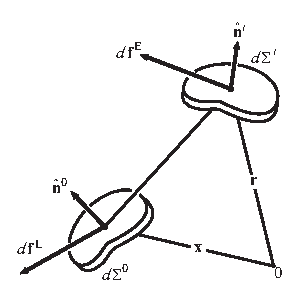
\includegraphics{../figures/chap02/fig05.eps}
\end{center}
\caption[twoforces]{\label{fig2.5}
表面力 $d\/{\bf f}^{\rm E}$ 和
$d\/{\bf f}^{\rm L}$ 分别作用在位于 $\bf r$ 的变形后的面积元 $\hat{\bf n}^t  d\/ \Sigma^t$ 上与位于
$\bf x$ 的变形前的面积元 $\hat{\bf n}^0  d\/ \Sigma^0$
上。}
\end{figure}
定义 $\bT^{\rm SK}$ 为
\eq
d\/\bef^{\rm L}=\bnh^0d\/\Sigma^0\cdot\bT^{\rm SK},
\en
我们看到第一类和第二类 Piola-Kirchhoff 应力之间的关系是
\eq
\label{2.TPKrelTSK}
\bT^{\rm SK}=\bT^{\rm PK}\cdot\bF^{-\rm T},\qquad
\bT^{\rm PK}=\bT^{\rm SK}\cdot\bF^{\rm T}.
\en
与式~(\ref{2.tpkt1}) 比较,
我们可以得到 $\bT^{\rm SK}$ 与拉格朗日柯西应力 $\bT^{\rm L}$ 之间的相互关系:
\eq
\label{2.tskt1}
\bT^{\rm SK}=J\,\bF^{-1}\cdot\bT^{\rm L}\cdot\bF^{-\rm T},\qquad
\bT^{\rm L}=J^{-1}\bF\cdot\bT^{\rm SK}\cdot\bF^{\rm T}.
\en
由于变换后的力 $d\/\bef^{\rm L}$ 可以被看作是作用在初始位置
$\bx$,而不是在移动后的位置 $\br$,
因此,第二类 Piola-Kirchhoff 应力 $\bT^{\rm SK}$ 是一个普通张量,而不是两点张量。
图~\ref{fig2.5} 显示了面积元 
$\bnh^t d\/\Sigma^t$ 和 $\bnh^0d\/\Sigma^0$
$\bnh^t d\/\Sigma^t$
与力 $d\/\bef^{\rm E}$ 和 $d\/\bef^{\rm L}$ 
之间的几何关系。
\index{stress!measures of|)}%
\index{tensor!stress|)}%
\index{stress tensor|)}%

\section{欧拉守恒定律}
\index{conservation law!Eulerian|(}%
\label{2.sec.euleq}

与前面一样,我们假定 $q^{\rm E}$ 是遍布于连续体内的 ``q量''
\index{q-stuff}%
的密度。
任一局地欧拉守恒定律的普遍形式是
\eq
\label{2.conslaw}
\p_t q^{\rm E} + \bdel_{\!\subr} \cdot \bk^{\rm E} = c^{\rm E}.
\en
其中 $\bk^{\rm E}$ 和 $c^{\rm E}$ 分别表示 ``q量'' 
在固定的 $\br$ 点在 $t$ 时刻的 {\em 通量\/} 
\index{q-stuff!flux of}%
\index{q-stuff!rate of creation of}%
与
{\em 生成率\/}。
通量 $\bk^{\rm E}$ 必须是比密度 $q^{\rm E}$ 或瞬时生成率 $c^{\rm E}$ 高一阶的张量。
如果将式~(\ref{2.conslaw}) 在一个
{\em 固定的\/} 体积 $V$ 内积分,并使用高斯定理,我们有
\index{volume!stationary}%
\index{stationary volume}%
\eq
\label{2.consint}
\frac{d}{dt} \int_V q^{\rm E}\,dV =
-\int_{\partial V} (\bnh \cdot \bk^{\rm E}) \,d\/\Sigma +
\int_V c^{\rm E}\,dV ,
\en
此处 $\p V$ 是 $V$ 的边界, $\bnh$ 
是向外的单位法向矢量。
式~(\ref{2.consint}) 证实了对守恒定律~(\ref{2.conslaw})
中 $\bk^{\rm E}$ 和 $c^{\rm E}$
两项的解释。
体积 $V$ 内 ``q量'' 的变化包含两项:
一项表面积分是因 ``q量'' 的通量 $\bk^{\rm E}$ 流过固定边界
$\p V$ 的部分,另一项体积分来自每一点处 ``q量'' 的生成率 $c^{\rm E}$。
表面积分前面的负号是因为 $\bnh$ 是 {\em 向外的\/} 单位法向矢量;
\index{outward normal}%
\index{unit normal}%
``q量'' 透过面积元 $\bnh \,d\/\Sigma$ {\em 流入\/} 体积 $V$ 
的速率是 $-(\bnh\cdot\bk^{\rm E})\,d\/\Sigma$。

\subsection{质量守恒}
\index{conservation!of mass!Eulerian|(}%
\index{mass!conservation of!Eulerian|(}%

形如~(\ref{2.conslaw}) 的最简单的定律是质量守恒定律;
我们用 $\rho^{\rm E}$ 表示质量密度。
由于质量不生不灭,移动体积 $V^t$ 内物体的总质量必须是常数:
\eq
\label{2.dtmass}
\frac{d}{dt} \int_{V^t} \rho^{\rm E}\,dV^t = 0.
\en
利用雷诺兹输运定理~(\ref{2.reynolds}),
我们可以把式~(\ref{2.dtmass}) 写成
\eq
\label{2.dtmass2}
\int_{V^t}[\p_t\rho^{\rm E} + \bdel_{\!\subr} \cdot
(\rho^{\rm E}\bu^{\rm E})]\,dV^t = 0.
\en
式~(\ref{2.dtmass2}) 必须对连续体中任意移动体积 $V^t$ 均成立;这一结果只有在被积函数恒等于零时才有可能:
\eq
\label{2.cont}
\p_t\rho^{\rm E} + \bdel_{\!\subr} \cdot (\rho^{\rm E}\bu^{\rm E}) = 0.
\en
这一欧拉形式的质量守恒定律被称为 {\em 连续性方程}。
\index{continuity equation}%
式~(\ref{2.cont}) 是普遍形式~(\ref{2.conslaw})
中取 $q^{\rm E}=\rho^{\rm E}$, $\bk^{\rm E}
=\rho^{\rm E}\bu^{\rm E}$ 和 $c^{\rm E}=0$ 的特例。

利用连续性方程,我们可以得到适用于任意广延
``q量'' 的另一种形式的雷诺兹输运定理。令 $\chi^{\rm E}$ 为该广延量的 {\em 密度比\/},
\index{q-stuff}%
\index{specific density}%
\index{density!specific}%
即单位质量而非单位体积的量,因而
\eq
\label{2.chidef}
q^{\rm E}=\rho^{\rm E}\chi^{\rm E}.
\en
将~(\ref{2.chidef})~代入~(\ref{2.reynolds}),并利用式 ~(\ref{2.Ddef})~和~(\ref{2.cont}),
我们得到
\eq
\label{2.Reynolds2}
\frac{d}{dt} \int_{V^t} \rho^{\rm E}\chi^{\rm E}\,dV^t =
\int_{V^t} \rho^{\rm E} D_t\chi^{\rm E}\,dV^t,
\en
下面我们将用此式来推导其余三个欧拉守恒定律。
我们也可以利用连续性方程将一般的守恒定律~(\ref{2.conslaw})
用物质导数 $D_t$ 来表示:
\eq
\label{2.conslaw2}
\rho^{\rm E} D_t\chi^{\rm E} + \bdel_{\!\subr}\cdot\bkappa^{\rm E}=c^{\rm E},
\en
其中
\eq
\bkappa^{\rm E}=\bk^{\rm E}-\bu^{\rm E}q^{\rm E}
=\bk^{\rm E}-\rho^{\rm E}\bu^{\rm E}\chi^{\rm E}.
\en
从物理上讲, $\bkappa^{\rm E}$ 这个量是 ``q量'' 相对于移动物体的通量;
总的欧拉通量 $\bk^{\rm E}$ 包含
{\em 平流\/}
\index{advection}%
\index{q-stuff!advection of}%
产生的通量
$\bu^{\rm E}q^{\rm E}
=\rho^{\rm E}\bu^{\rm E}\chi^{\rm E}$
加上相对通量 $\bkappa^{\rm E}$。
质量的通量完全是平流的:
$\chi^{\rm E}=1$ 和 $\bkappa^{\rm E}=\bzero$,
因此~(\ref{2.conslaw2}) 变得多余了。

用物质导数 $D_t$ 也可以将连续性方程
~(\ref{2.cont})
写成如下形式
\eq
\label{2.cont2}
D_t\rho^{\rm E}+\rho^{\rm E}\bdel_{\!\subr}\cdot\bu^{\rm E}=0.
\en
式~(\ref{2.cont2}) 给出了欧拉速度散度的物理解释,
\index{divergence!of the velocity}%
即欧拉应变率张量的迹: $\bdel_{\!\subr}\cdot\bu^{\rm E}={\rm tr} \,\bD^{\rm E}$。
定义 {\em 体积比\/}
\index{specific volume}%
\index{volume!specific}%
$\tau^{\rm E}$ 为
\eq
\rho^{\rm E}\tau^{\rm E}=1,
\en
我们看到
\eq
\label{2.divdef}
\bdel_{\!\subr}\cdot\bu^{\rm E} = -\frac{D_t\rho^{\rm E}}{\rho^{\rm E}}
= \frac{D_t\tau^{\rm E}}{\tau^{\rm E}}.
\en
显然, $\bdel_{\!\subr}\cdot\bu^{\rm E}$ 
是在 $t$ 时刻位于 $\br$ 处的质点其单位质量的分数体积变化率。  对于 {\em 不可压缩的\/}
\index{incompressible material}%
物体,其组成质点具有恒定的体积:
$\bdel_{\!\subr}\cdot\bu^{\rm E}=0$。
\index{conservation!of mass!Eulerian|)}%
\index{mass!conservation of!Eulerian|)}%

\subsection{动量守恒}
\index{conservation!of momentum!Eulerian|(}%
\index{momentum!conservation of!Eulerian|(}%

惯性参照系内一团移动物体的{\em 牛顿第二定律} 
\index{Newton's second law}%
是
\eq
\label{2.Newton}
\frac{d}{dt} \int_{V^t} \rho^{\rm E}\bu^{\rm E}\,dV^t = \bsF,
\en
其中 $\bsF$ 是作用在移动中体积 $V^t$ 上的总外力。
力 $\bsF$ 包括了透过边界 $\p V^t$ 作用的 {\em 短程表面力\/}
\index{force!short-range}%
\index{short-range force}%
$\bsF_{\rm s}$ 以及作用在体积 $V^t$ 内部所有质点上的 {\em 长程体力\/} $\bsF_{\rm b}$:
\index{force!long-range}%
\index{long-range force}%
\eq
\bsF = \bsF_{\rm s} + \bsF_{\rm b}.
\en
其中表面力可以利用作用在边界上的柯西应力 $\bT^{\rm E}$ 写成
\eq
\label{2.Fsurf}
\bsF_{\rm s}=\int_{\partial V^t}(\bnh^t\cdot\bT^{\rm E})\,d\/\Sigma^t=
\int_{V^t}(\bdel_{\!\subr}\cdot\bT^{\rm E})\,dV^t,
\en
上式中第二个等号可以从高斯定理得到。
我们假定长程体力 $\bsF_{\rm b}$ 可以通过一个特定的体力密度
$\bg^{\rm E}$ 表示为
\eq
\label{2.Fbody}
\bsF_{\rm b}=\int_{V^t} \rho^{\rm E}\bg^{\rm E}\,dV^t.
\en
典型的长程力当然是引力;
与其相应的 $\bg^{\rm E}$ 则是 $t$ 时刻在 $\br$ 处的
{\em 重力场\/}。
\index{gravitational field}%

将式~(\ref{2.Fsurf})~和~(\ref{2.Fbody})
代入式~(\ref{2.Newton}), 再利用~(\ref{2.Reynolds2}) 形式的雷诺兹输运定理,我们有
\eq
\label{2.Newton2}
\int_{V^t}[\rho^{\rm E}D_t\bu^{\rm E} -\bdel_{\!\subr}\cdot\bT^{\rm E}
-\rho^{\rm E}\bg^{\rm E}]\,dV^t = \bzero.
\en
由于式~(\ref{2.Newton2}) 对连续体中任意移动中体积都成立,因此被积函数必须恒等于零;
因而欧拉形式的动量守恒定律成为
\eq
\label{2.momeqn}
\rho^{\rm E}D_t\bu^{\rm E}
=\bdel_{\!\subr}\cdot\bT^{\rm E}+\rho^{\rm E}\bg^{\rm E}.
\en
式~(\ref{2.momeqn}) 是一般形式~(\ref{2.conslaw2}) 取 $\chi^{\rm E}=\bu^{\rm E}$,
$\bkappa^{\rm E}=-\bT^{\rm E}$ 和 $c^{\rm E}=\rho^{\rm E}\bg^{\rm E}$ 的特例。
其中应力张量的符号是因为我们约定了式~(\ref{2.TEdef}) 中的 $d\/\bef^{\rm E}$ 是 {\em 由\/} 表面面积元 
$\bnh^td\/\Sigma^t$ {\em 正面\/} 
的质点 {\em 对\/} 其 {\em 背面\/} 质点的作用力。
依照这个约定, {\em 负的\/} 柯西应力
$-\bT^{\rm E}$ 可以被看作是相对于移动中物体的动量通量;
相对于惯性空间的通量则是
$\bk^{\rm E}=\rho^{\rm E}\bu^{\rm E}\bu^{\rm E}-\bT^{\rm E}$。
为简洁起见,我们称守恒定律~(\ref{2.momeqn}) 为
{\em 动量方程}。
\index{momentum equation}%
\index{conservation!of momentum!Eulerian|)}%
\index{momentum!conservation of!Eulerian|)}%

\subsection{角动量守恒}
\index{conservation!of angular momentum!Eulerian|(}%
\index{angular momentum!conservation of!Eulerian|(}%

一团物体的角动量变化率必须等于外来力矩的和。
忽略任何可能的内部角动量以及任何与固有自转相关的面力矩与体力矩,我们有
\eq
\label{2.angmom}
\frac{d}{dt}\int_{V^t}\rho^{\rm E}(\br\times\bu^{\rm E})\,dV^t
=\bsN_{\rm s}+\bsN_{\rm b}.
\en
其中 $\bsN_{\rm s}$ 和 $\bsN_{\rm b}$ 分别为
作用在 $V^t$ 上的表面力和体力所产生的力矩:
\index{torque}%
\eqa
\label{2.Nsurf}
\lefteqn{\bsN_{\rm s} =\int_{\partial V^t} \br\times(\bnh^t\cdot
\bT^{\rm E})\,d\/\Sigma^t=-\int_{\partial V^t}(\bnh^t\cdot\bT^{\rm E})\times\br
\,d\/\Sigma^t} \nonumber \\
&&\mbox{}\!\!\!=-\int_{\partial V^t}\bnh\cdot(\bT^{\rm E}\times\br)
\,d\/\Sigma^t=-\int_{V^t}\bdel_{\!\subr}\cdot(\bT^{\rm E}
\times\br)\,dV^t,
\ena
\eq
\label{2.Nbody}
\bsN_{\rm b}=\int_{V^t}\rho^{\rm E}(\br\times\bg^{\rm E})\,dV^t.
\en
将式~(\ref{2.Nsurf})~和~(\ref{2.Nbody})~代入~(\ref{2.angmom}),再使用~(\ref{2.Reynolds2}) 形式的输运定理,我们得到
\eq
\int_{V^t}[\rho^{\rm E}D_t(\br\times\bu^{\rm E})+\bdel_{\!\subr}\cdot
(\bT^{\rm E}\times\br)-\rho^{\rm E}(\br\times\bg^{\rm E})]\,dV^t=\bzero,
\en
同样,由于 $V^t$ 是任意的移动中体积,被积函数必须恒等于零;
因而我们得到角动量守恒定律
\eq
\label{2.angmom2}
\rho^{\rm E}D_t(\br\times\bu^{\rm E})+\bdel_{\!\subr}\cdot
(\bT^{\rm E}\times\br)=\rho^{\rm E}(\br\times\bg^{\rm E}).
\en
式~(\ref{2.angmom2}) 的结果是在欧拉形式~(\ref{2.conslaw2})中
取 $\chi^{\rm E}=\br\times\bu^{\rm E}$, $\bkappa^{\rm E}=\bT^{\rm E}\times\br$
和 $c^{\rm E}=\rho^{\rm E}(\br\times\bg^{\rm E})$;
相对于惯性空间的角动量总通量是
$\bk^{\rm E}=\rho^{\rm E}\bu^{\rm E}
(\br\times\bu^{\rm E})+\bT^{\rm E}\times\br$.

经过合并同类项,并考虑到 $(D_t\br)\times\bu^{\rm E}=
\bu^{\rm E}\times\bu^{\rm E}=\bzero$,我们可以将~(\ref{2.angmom2})
表示成
\eq
\label{2.angmom3}
\br\times(\rho^{\rm E}D_t\bu^{\rm E}
-\bdel_{\!\subr}\cdot\bT^{\rm E}-\rho^{\rm
E}\bg^{\rm E}) -\wedge\bT^{\rm E}=\bzero.
\en
根据动量方程~(\ref{2.momeqn}),式~(\ref{2.angmom3}) 中括号内的表达式恒等于零;
因此角动量守恒定律可以简化为
\eq
\label{2.angmom4}
\wedge\bT^{\rm E}=\bzero.
\en
式~(\ref{2.angmom4}) 确保了柯西应力
$\bT^{\rm E}$ 必须是 {\em 对称的\/}:
\index{stress!Cauchy!symmetry of}%
\index{Cauchy stress!symmetry of}%
\eq
\label{2.TEsymm}
(\bT^{\rm E})^{\rm T}=\bT^{\rm E}.
\en
上式为无自转或 {\em 无极性\/}
\index{non-polar continuum}%
\index{continuum!non-polar}%
连续体角动量守恒定律的最常见形式。
利用对称性~(\ref{2.TEsymm}),
角动量通量可以表示成另一种形式 $\bk^{\rm E}=\rho^{\rm E}\bu^{\rm E}
(\br\times\bu^{\rm E})-\br\times\bT^{\rm E}$。
\index{conservation!of angular momentum!Eulerian|)}%
\index{angular momentum!conservation of!Eulerian|)}%

\subsection{能量守恒}
\index{conservation!of energy!Eulerian|(}%
\index{energy!conservation of!Eulerian|(}%

要建立普遍的能量守恒定律必须明确地将热作为一种能量来对待;
为此我们需要引入一些热力学的概念。
宏观的动能密度
$\half\rho^{\rm E}(\bu^{\rm E}\cdot\bu^{\rm E})$ 并不是连续体内唯一的能量形式;实际的物体还可以储存并输运热能以及原子之间的势能。
我们将这种热动力学 {\em 内能} 
\index{energy!internal}%
\index{internal energy density}%
的密度用 $U^{\rm E}$ 来表示; 而总的欧拉能量密度为 $\rho^{\rm E}(\half\bu^{\rm E}\cdot\bu^{\rm E}+U^{\rm E})$。
因物质的平流而产生的欧拉内能通量是 $\rho^{\rm E}U^{\rm E}\bu^{\rm E}$;此外,内能还可以通过热传导过程输运出入物体。
我们用 $\bH^{\rm E}$ 表示欧拉热通量矢量;
\index{heat flux}%
而热能或内能的总通量是 $\rho^{\rm E}U^{\rm E}\bu^{\rm E}+\bH^{\rm E}$。
我们要引入的最后一个热动力学量是内部生热率 $h^{\rm E}$; 它用在普遍公式中来代表由微观过程如放射性衰变带来的贡献。
 
适用于一个移动中体积 $V^t$ 的能量守恒定律有如下形式
\eqa
\label{2.energy}
\lefteqn{\frac{d}{dt}\int_{V^t}\rho^{\rm E}
(\half\bu^{\rm E}\cdot\bu^{\rm E}+U^{\rm E})
\,dV^t} \nonumber \\
& & \mbox{} = \int_{V^t}\rho^{\rm E}\bg^{\rm E}\cdot\bu^{\rm E}\,dV^t
\,+\int_{\partial V^t}
(\bnh^t\cdot\bT^{\rm E})\cdot\bu^{\rm E}\,d\/\Sigma^t \nonumber \\
& & \mbox{} \qquad\quad+ \int_{V^t}\rho^{\rm E}h^{\rm E}\,dV^t\,-
\int_{\partial V^t}(\bnh^t\cdot\bH^{\rm E})\,d\/\Sigma^t.
\ena
式~(\ref{2.energy}) 左边的量代表的是体积内总能量变化率,包括动能与内能;右边的四项代表能够改变该能量的各种方式。
前两个积分表示通过体力与面力的作用能够给该体积带来的机械能的增加率,而后两个积分则是由内部生热和热传导而带来的热能的增加率。最后一项前面的负号是由于根据定义
$(\bnh^t\cdot\bH^{\rm E})\,d\/\Sigma^t$ 是热能从面元 $\bnh^t\,d\/\Sigma^t$ 的背面传导到正面的速率。
将高斯定理和雷诺兹定理用于式~(\ref{2.Reynolds2}),我们得到
\eqa
\label{2.TOTENER}
\lefteqn{\int_{V^t}[\rho^{\rm E}
D_t(\half\bu^{\rm E}\cdot\bu^{\rm E}+U^{\rm E})} \nonumber \\
&&\mbox{}\frac{}{}+\bdel_{\!\subr}\cdot(\bH^{\rm E}
-\bT^{\rm E}\cdot\bu^{\rm E})
-\rho^{\rm E}(h^{\rm E}+\bg^{\rm E}\cdot\bu^{\rm
E})]\,dV^t=\bzero.
\ena
令~(\ref{2.TOTENER}) 中的被积函数为零,
然后用从~(\ref{2.angmom2})~到~(\ref{2.angmom3})
同样的做法消去其中隐含的动量方程,
再利用对称性~(\ref{2.TEsymm}),
我们得到欧拉能量守恒定律:
\eq
\label{2.inteneqn}
\rho^{\rm E}D_tU^{\rm E}+ \bdel_{\!\subr}\cdot\bH^{\rm E}=
\bT^{\rm E}\!:\!\bD^{\rm E}+\rho^{\rm E}h^{\rm E}.
\en
式~(\ref{2.inteneqn})称作
{\em 内能方程},
\index{internal-energy equation}%
它是一般式~(\ref{2.conslaw2}) 取 $\chi^{\rm E}=U^{\rm E}$ 和
$\bkappa^{\rm E}=\bH^{\rm E}$ 的特例。单位体积里的内能由机械过程产生或因放射性衰变而“生成”的速率是
$c^{\rm E}=\bT^{\rm E}\!:\!\bD^{\rm E}+\rho^{\rm E}h^{\rm E}$。

所有地震现象的时间和空间尺度决定了在一个振荡周期内从压缩传到扩张区域的热是可以忽略不计的。
要看清这一点,我们将一个时间段 $T$ 内热传输过的距离 $L_{\rm heat}\approx\sqrt{\kappa T}$
与地震波传播的距离
$L_{\rm wave}\approx vT$ 做一个比较。
显然,在振荡周期 $T\gg \kappa v^{-2}$ 时,
$L_{\rm heat}\ll L_{\rm wave}$。
将上地幔普遍的热扩散系数 $\kappa$ 和 P波波速度 $v$ 代入,我们发现热流只有对超短周期的地震波
$\kappa v^{-2}\approx 10^{-14}$~秒才是重要的。
在地震学中,我们所关心的波的周期通常都大于
$T\approx 10^{-2}$~秒;
因此把形变看做 {\em 绝热\/}
过程是一个很好的近似:
\index{deformation!adiabatic}%
\index{adiabatic deformation}%
\eq \label{2.noheat}
\bH^{\rm E}=\bzero.
\en
在地震学的时间尺度上放射性生热也是完全可以忽略的,因此我们设定 $h^{\rm E}=0$。 经过这些简化,在所有地震学感兴趣的问题中内能方程变为
\eq
\label{2.inteneqn2}
\rho^{\rm E}D_tU^{\rm E}=\bT^{\rm E}\!:\!\bD^{\rm E}.
\en
在一个闭合的形变周期内为克服应力所做的机械功严格来说一般是正的,即
\eq
\label{2.POSWORK}
\oint \bT^{\rm E}\!:\!\bD^{\rm E}\,dt \geq 0,
\en
这反映了在任意实际的物体中内摩擦过程从本质上讲都是耗散性的。
只有在完全弹性连续体这一理想情况下所做的功才是
{\em 可恢复的\/},只有此时
\index{work!recoverable}%
\index{recoverable work}%
式~(\ref{2.POSWORK}) 中的等号才会成立。
\index{conservation!of energy!Eulerian|)}%
\index{energy!conservation of!Eulerian|)}%

\subsection{边界条件}
\index{boundary conditions!Eulerian|(}%

前面所推导出的质量、动量、角动量和能量的守恒定律还必须结合在分隔两个不同物体的边界上的连续性条件才行。
在本书中,我们用符号 $[q]^+_-$ 来表示物理量 $q$ 从一个边界的正 $+$ 面到背 $-$ 面在数值上的跳跃。

在两个固体之间密切接合的边界上,欧拉速度必须连续:
\eq
\label{2.weldbc}
[\bu^{\rm E}]^+_-=\bzero.
\en
在固体与非粘滞性流体间的边界上,以及分隔两个固体的理想断层面上,切向的滑动是允许的。
在这种滑动边界上,式~(\ref{2.weldbc}) 由下式取代
\eq
\label{2.slipbc}
[\bnh^t\cdot\bu^{\rm E}]^+_-=0,
\en
其中 $\bnh^t$ 是边界面的单位法向矢量。
式~(\ref{2.slipbc}) 保证了在边界处两种介质之间既没有分离也没有相互穿透。

除了上述两个运动学条件之外,在密接和滑动边界上还有一个牵引力 $\bnh^t\cdot\bT^{\rm E}$ 必须连续的动力学条件:
\eq
\label{2.stressbc}
[\bnh^t\cdot\bT^{\rm E}]^+_-=\bzero.
\en
最后,在固体和非粘滞性流体之间的边界上不能有切向牵引力,即在一个无摩擦力的固-液边界上
$\bnh^t\cdot\bT^{\rm E}$ 的方向必须与瞬时法向矢量
$\bnh^t$
一致:
\eq
\label{2.stressfs}
\bnh^t\cdot\bT^{\rm E}=\bnh^t(\bnh^t\cdot\bT^{\rm E}\cdot\bnh^t).
\en
上述四个条件(\ref{2.weldbc})--(\ref{2.stressfs})
适用于瞬时的边界位置,即在 $t$ 时刻的边界上的所有点
$\br$ 都必须满足这些条件。
\index{boundary!deformed}%
\index{deformed boundary}%
\index{boundary conditions!Eulerian|)}%

\subsection{转动参照系}
\index{rotation!reference frame|(}%
\index{reference frame|(}%

现在假设我们不是在惯性系中来观察运动,而是在一个以恒定的角速度
$\bOmega$ 相对于惯性系转动的参照系里。质量与内能守恒定律、柯西应力的对称性以及运动学和动力学边界条件均不受这一参照系改变的影响。
但是,动量方程~(\ref{2.momeqn}) 必须做修改以纳入 {\em 科里奥利\/}
\index{Coriolis acceleration}%
\index{acceleration!Coriolis}%
和 {\em 向心\/} 两种视加速度:
\index{centripetal acceleration}%
\index{acceleration!centripetal}%
\eq
\label{2.momeqn2}
\rho^{\rm E}[D_t\bu^{\rm E}+2\bOmega\times\bu^{\rm E}+\bOmega\times
(\bOmega\times\br)]=\bdel_{\!\subr}\cdot\bT^{\rm E}
+\rho^{\rm E}\bg^{\rm E}.
\en
由于地震仪总是在地球的周日自转所产生的科里奥利和向心加速度的作用下,我们很自然地使用转动参照系来分析地球对地震或其它加载现象的弹性-引力响应。
为考虑转动,在本章的剩余部分以及下一章我们将使用式
~(\ref{2.momeqn2})
而不是~(\ref{2.momeqn})。

\index{rotation!reference frame|)}%
\index{reference frame|)}%
\index{conservation law!Eulerian|)}%

\section{拉格朗日守恒定律}
\index{conservation law!Lagrangian|(}%
\label{2.sec.lageq}

前面讨论的四个欧拉守恒定律每一个都有相对应的拉格朗日形式,这是我们下一步要考虑的。
在推导欧拉守恒定律时,我们都是首先用一个任意移动中的体积来建立积分形式的平衡原理,然后再把积分号“涂掉”。
我们将用类似的方法来推导拉格朗日定律,首先寻求用初始形态的
{\em 变形前\/}体积 $V^0$ 来建立积分形式的平衡原理。
\index{undeformed volume}%
\index{volume!undeformed}%

\subsection{质量守恒}
\index{conservation!of mass!Lagrangian|(}%
\index{mass!conservation of!Lagrangian|(}%

利用空间坐标 $\br$ 与物质坐标 $\bx$ 之间的变换关系,移动中体积
$V^t$ 内的质量可以表示成在变形前体积
$V^0$ 上的积分:
\eq
\int_{V^t}\rho^{\rm E}\,dV^t=\int_{V^0}\rho^{\rm L}J\,dV^0,
\en
其中 $J$ 是该坐标变换的雅可比矩阵。
由于质量不生不灭,在任何 $t$ 时刻的体积内的质量必须等于
$t=0$ 时刻体积内的质量:
\eq
\label{2.rhoLJ}
\int_{V^0}\rho^{\rm L}J\,dV^0=\int_{V^0}\rho^0\,dV^0,
\en
这里 $\rho^0(\bx)=\rho^{\rm L}(\bx,0)$。
式~(\ref{2.rhoLJ}) 必须对初始形态中的任意体积 $V^0$
均成立;而这只有在左右两边的被积函数处处相等时才能满足,即:
\eq
\label{2.lagmass}
\rho^{\rm L}J=\rho^0.
\en
这就是拉格朗日形式的质量守恒定律,它建立了质点的瞬时密度
$\rho^{\rm L}$ 与其初始密度 $\rho^0$ 之间的关系。

拉格朗日形式的质点体积比仍然定义为
$\tau^{\rm L}(\bx,t)=\tau^{\rm E}(\br(\bx,t),t)$,或者等效为
$\rho^{\rm L}\tau^{\rm L}=1$。
用 $\tau^{\rm L}$ 而非 $\rho^{\rm L}$,
式~(\ref{2.lagmass}) 变成
\eq
\label{2.tauLJ}
\tau^{\rm L}=J\tau^0,
\en
其中 $\tau^0(\bx)=\tau^{\rm L}(\bx,0)$。
式~(\ref{2.tauLJ}) 实际上就是以不同的符号来表示的微分体积的关系 $dV^t=J\,dV^0$。

与利用欧拉形式~(\ref{2.cont})把雷诺兹输运定理改写成~(\ref{2.Reynolds2})的形式一样,
我们也可以用拉格朗日质量守恒律~(\ref{2.lagmass})
来改写任意 ``q量'' 的变换公式。
\index{q-stuff}%
一个移动中体积 $V^t$ 内部总的
``q量'' 可以写成体积 $V^0$ 内的积分形式
\eq
\label{2.chiEL}
\int_{V^t}\rho^{\rm E}\chi^{\rm E}\,dV^t=\int_{V^0}\rho^0\chi^{\rm L}\,dV^0,
\en
其中 $\chi^{\rm L}(\bx,t)=\chi^{\rm E}(\br(\bx,t),t)$ 是密度比。下面我们将利用~(\ref{2.chiEL}) 来推导拉格朗日形式的动量与能量守恒定律。
\index{conservation!of mass!Lagrangian|)}%
\index{mass!conservation of!Lagrangian|)}%

\subsection{动量守恒}
\index{conservation!of momentum!Lagrangian|(}%
\index{momentum!conservation of!Lagrangian|(}%

我们考虑任意移动中体积 $V^t$ 的欧拉动量方程
~(\ref{2.momeqn2}) 的积分。将所有与密度
$\rho^{\rm E}$ 成比例的项移到左边,并利用高斯定理,我们得到
\eqa
\label{2.Newton3}
\lefteqn{\int_{V^t}\rho^{\rm E}[D_t\bu^{\rm E}+2\bOmega\times\bu^{\rm E}
+\bOmega\times(\bOmega\times\br)-\bg^{\rm E}]\,dV^t}
\nonumber \\
&&=\int_{\partial V^t}(\bnh^t\cdot\bT^{\rm E})\,d\/\Sigma^t.
\ena
左边的量可以利用式~(\ref{2.chiEL}) 
变换为在变形前体积 $V^0$
上的积分:
\eqa
\label{2.laglhs}
\lefteqn{\int_{V^t}\rho^{\rm E}[D_t\bu^{\rm E}+2\bOmega\times\bu^{\rm E}
+\bOmega\times(\bOmega\times\br)-\bg^{\rm
E}]\,dV^t} \nonumber \\
&&\mbox{}=\int_{V^0}\rho^0[\p_t^2\br+2\bOmega\times\p_t\br
+\bOmega\times(\bOmega\times\br)-\bg^{\rm L}]\,dV^0,
\ena
其中 $\bg^{\rm L}(\bx,t)=\bg^{\rm E}(\br(\bx,t),t)$。
右边的面积分也可以用~(\ref{2.TPKdef}) 所定义的第一类
Piola-Kirchhoff 应力张量变换为:
\eqa
\label{2.lagrhs}
\lefteqn{
\int_{\partial V^t}(\bnh^t\cdot\bT^{\rm E})\,d\/\Sigma^t
=\int_{\partial V^0}(\bnh^0\cdot\bT^{\rm PK})\,d\/\Sigma^0} \nonumber \\
&&\mbox{}=\int_{V^0}(\bdel_{\!\subx}\cdot\bT^{\rm PK})\,dV^0,
\ena
其中第二个等号是通过在变形前体积
$V^0$ 上使用高斯定理得到的。
结合式~(\ref{2.laglhs})~和~(\ref{2.lagrhs}),我们可以把平衡原理~(\ref{2.Newton3}) 写成如下形式
\eqa
\label{2.Newton4}
\lefteqn{\int_{V^0}\{\rho^0[\p_t^2\br+2\bOmega\times\p_t\br
+\bOmega\times(\bOmega\times\br)]} \nonumber \\
&&\qquad\qquad\qquad
\mbox{}-\bdel_{\!\subx}\cdot\bT^{\rm PK}
-\rho^0\bg^{\rm L}\}\,dV^0=\bzero.
\ena
由于体积 $V^0$ 是任意的,~(\ref{2.Newton4}) 中的被积函数必须恒等于零,因而我们得到均匀转动参照系中拉格朗日形式的动量方程
\eq
\label{2.lagmomeqn}
\rho^0[\p_t^2\br+2\bOmega\times\p_t\br
+\bOmega\times(\bOmega\times\br)]=\bdel_{\!\subx}
\cdot\bT^{\rm PK}+\rho^0\bg^{\rm L}.
\en
值得注意的是,~(\ref{2.momeqn2}) 中欧拉柯西应力的散度
$\bdel_{\!\subr}\cdot\bT^{\rm E}$ 变换成为~(\ref{2.lagmomeqn}) 中的第一类
Piola-Kirchhoff 应力的散度 $\bdel_{\!\subx}\cdot\bT^{\rm PK}$;
事实上,
当初对 $\bT^{\rm PK}$ 的定义~(\ref{2.TPKdef}) 就是为了实现这一简单的变换。

拉格朗日形式的动量方程也可以用第二类Piola-Kirchhoff 应力 $\bT^{\rm SK}$
而不是 $\bT^{\rm PK}$ 来表示;将关系式~(\ref{2.TPKrelTSK})~代入~(\ref{2.lagmomeqn})
我们有
\eqa
\label{2.lagmomeqn2}
\lefteqn{\rho^0[\p_t^2\br+2\bOmega\times\p_t\br
+\bOmega\times(\bOmega\times\br)]} \nonumber \\
&&\mbox{}\qquad\qquad=\bdel_{\!\subx}\cdot
(\bT^{\rm SK}\cdot\bF^{\rm T})+\rho^0\bg^{\rm L}.
\ena
式~(\ref{2.lagmomeqn2}) 中的应力散度项比
~(\ref{2.lagmomeqn}) 中的更复杂;相反,我们下面会看到,角动量守恒定律用 $\bT^{\rm SK}$ 表示要比用 $\bT^{\rm PK}$ 更简单。
\index{conservation!of momentum!Lagrangian|)}%
\index{momentum!conservation of!Lagrangian|)}%

\subsection{角动量守恒}
\index{conservation!of angular momentum!Lagrangian|(}%
\index{angular momentum!conservation of!Lagrangian|(}%
\index{stress!first Piola-Kirchhoff!asymmetry of|(}%
\index{Piola-Kirchhoff stress!first!asymmetry of|(}%
\index{stress!second Piola-Kirchhoff!symmetry of|(}%
\index{Piola-Kirchhoff stress!second!symmetry of|(}%
\label{2.sec.lagangmom}

第一类 Piola-Kirchhoff 应力 $\bT^{\rm PK}$ 与其转置
$(\bT^{\rm PK})^{\rm T}$ 之间有关系
\eq
\label{2.TPKtr}
(\bT^{\rm PK})^{\rm T}=\bF\cdot\bT^{\rm PK}\cdot\bF^{-\rm T}.
\en
式~(\ref{2.TPKtr}) 可以很容易地结合关系式~(\ref{2.tpkt1})
与拉格朗日柯西应力的对称性
$(\bT^{\rm L})^{\rm T}=\bT^{\rm L}$ 得到证明。
相反,利用~(\ref{2.tskt1}),我们发现如果 $\bT^{\rm L}$ 是对称的,那么第二类
Piola-Kirchhoff 应力 $\bT^{\rm SK}$ 也是对称的:
\eq
\label{2.TSKtr}
(\bT^{\rm SK})^{\rm T}=\bT^{\rm SK}.
\en
式~(\ref{2.TPKtr})~和~(\ref{2.TSKtr}) 就是拉格朗日形式的角动量守恒定律。

严格来说,从关系式~(\ref{2.TPKtr}) 我们不能对
$\bT^{\rm PK}$ 是否对称下任何结论。
如果我们坚持把第一类 Piola-Kirchhoff 应力看作是一个两点张量,那么对称这个概念是毫无意义的,因为 $\bT^{\rm PK}$ 与其转置 $(\bT^{\rm PK})^{\rm T}$
是在不同的空间里。不过,我们将如同对待形变张量 $\bF$ 
一样,不去考虑 $\bT^{\rm PK}$ 的两点特性;
因此我们说,基于式~(\ref{2.TPKtr}),
{\em 第一类 Piola-Kirchhoff 应力是不对称的}.
\index{stress!first Piola-Kirchhoff!asymmetry of|)}%
\index{Piola-Kirchhoff stress!first!asymmetry of|)}%
\index{stress!second Piola-Kirchhoff!symmetry of|)}%
\index{Piola-Kirchhoff stress!second!symmetry of|)}%
\index{conservation!of angular momentum!Lagrangian|)}%
\index{angular momentum!conservation of!Lagrangian|)}%

\subsection{能量守恒}
\index{conservation!of energy!Lagrangian|(}%
\index{energy!conservation of!Lagrangian|(}%

对绝热内能方程~(\ref{2.inteneqn2}) 在任意移动中体积 $V^t$ 上积分,我们得到
\eq
\label{2.inteneqn3}
\int_{V^t}\rho^{\rm E}D_tU^{\rm E}\,dV^t=
\int_{V^t}\bT^{\rm E}\!:\!\bD^{\rm E}\,dV^t.
\en
利用式~(\ref{2.chiEL}),上式左边可以变换为在变形前体积
$V^0$ 上的积分:
\eq
\label{2.UEULrel}
\int_{V^t}\rho^{\rm E}D_tU^{\rm E}\,dV^t=
\int_{V^0}\rho^0\p_tU^{\rm L}\,dV^0.
\en
在对右边做变换时,我们必须先把内能的机械生成率
$\bT^{\rm E}\!:\!\bD^{\rm E}$ 用第一和第二类 Piola-Kirchhoff 应力 $\bT^{\rm PK}$ 和 $\bT^{\rm SK}$ 来表示。利用式~(\ref{2.FrelG2})~和~(\ref{2.tpkt1}),我们得到
\eqa
\label{2.workrate}
\lefteqn{\bT^{\rm E}\!:\!\bD^{\rm E}=\bT^{\rm E}\!:\!\bG^{\rm E}={\rm tr}\,
[J^{-1}(\bF\cdot\bT^{\rm PK})\cdot(\p_t\bF\cdot\bF^{-1})]}
\nonumber \\
&&\quad\,\,\,\,=J^{-1}\,{\rm tr}\,(\bT^{\rm PK}\cdot\p_t\bF)
=J^{-1}(\bT^{\rm PK}\!:\!\p_t\bF^{\rm T}).
\ena
而如果用~(\ref{2.DEdtEL})~和~(\ref{2.tskt1}),
我们得到另一个形式
\eqa
\label{2.workrate2}
\lefteqn{\bT^{\rm E}\!:\!\bD^{\rm E}=
{\rm tr}\,[J^{-1}(\bF\cdot\bT^{\rm SK}\cdot\bF^{\rm T})
\cdot(\bF^{-\rm T}\cdot\p_t\bE^{\rm L}\cdot\bF^{-1})]}
\nonumber \\
&&\quad\,\,\,\,=J^{-1}\,{\rm tr}\,(\bT^{\rm SK}\cdot\p_t\bE^{\rm L})
=J^{-1}(\bT^{\rm SK}\!:\!\p_t\bE^{\rm L}).
\ena
将以上两个表达式代入~(\ref{2.inteneqn3}) 的左边,经过变换并与~(\ref{2.UEULrel}) 结合,我们有
\eq
\label{2.inteneqn4}
\int_{V^0}[\rho^0\p_tU^{\rm L}-\bT^{\rm PK}\!:\!\p_t\bF^{\rm T}]\,dV^0=0,
\en
\eq
\label{2.inteneqn5}
\int_{V^0}[\rho^0\p_tU^{\rm L}-\bT^{\rm SK}\!:\!\p_t\bE^{\rm L}]\,dV^0=0.
\en
由于式~(\ref{2.inteneqn4})~和~(\ref{2.inteneqn5})
中的体积都是任意的,被积函数必须为零;
因而拉格朗日绝热内能方程可以写成两个等价形式之一
\eq
\label{2.inteneqn6}
\rho^0\p_tU^{\rm L}=\bT^{\rm PK}\!:\!\p_t\bF^{\rm T}
=\bT^{\rm SK}\!:\!\p_t\bE^{\rm L}.
\en
在形变的一个闭合周期内克服 $\bT^{\rm PK}$ 或
$\bT^{\rm SK}$ 所做的功本质上是耗散性的,即
\eq
\oint\bT^{\rm PK}\!:\!\p_t\bF^{\rm T}\,dt
=\oint\bT^{\rm SK}\!:\!\p_t\bE^{\rm L}\,dt \geq 0,
\en
其中等号仍然是在完全弹性介质的情况才成立的。
在第~\ref{2.sec.constrel}节中,我们将借助
式~(\ref{2.inteneqn6}) 来讨论完全弹性介质的本构关系。
\index{conservation!of energy!Lagrangian|)}%
\index{energy!conservation of!Lagrangian|)}%

\subsection{边界条件}
\index{boundary conditions!Lagrangian|(}%

在 $t=0$ 时刻叠置在一个密接边界两侧的质点必须始终保持叠置在一起;因此拉格朗日形式的运动学边界条件可以简单地表示成
\eq
\label{2.lagkbc}
[\br]^+_-=\bzero.
\en
密接边界的动力学边界条件~(\ref{2.stressbc}) 也可以直接用第一类 Piola-Kirchhoff 应力表示成:
\eq
\label{2.lagsbc}
[\bnh^0\cdot\bT^{\rm PK}]^+_-=\bzero,
\en
这里我们用到了等式
$\bnh^t\cdot\bT^{\rm E}\,d\/\Sigma^t=
\bnh^0\cdot\bT^{\rm PK}\,d\/\Sigma^0$ 以及微分面元 $d\/\Sigma^t$
和 $d\/\Sigma^0$ 的连续性条件。  (\ref{2.lagkbc})~和~(\ref{2.lagsbc}) 这两个拉格朗日连续条件都是施加在初始形态中 {\em 变形前的\/} 边界上的,
\index{boundary!undeformed}%
\index{undeformed boundary}%
相反地,
欧拉条件~(\ref{2.weldbc})--(\ref{2.stressfs})
则是施加在当前形态中 {\em 变形后的\/}边界上。
在固-液边界或断层边界上,由于切向滑动的存在,两个条件均不成立;我们到第3.4节再来考虑这种滑动边界上的拉格朗日边界条件。
\index{boundary conditions!Lagrangian|)}%
\index{conservation law!Lagrangian|)}%

\section{引力势理论}
\index{gravitational potential|(}%

由于引力是一种 {\em 保守\/}力,
\index{force!conservative}%
\index{conservative force}%
我么可以把单位质量的欧拉引力 $\bg^{\rm E}$ 表示成 {\em 欧拉引力势函数\/} 
\index{gravitational potential!Eulerian}%
$\phi^{\rm E}$ 的梯度:
\eq
\label{2.phiEdef}
\bg^{\rm E}=-\bdel_{\!\subr}\phi^{\rm E}.
\en
由于式~(\ref{2.phiEdef}) 中的负号,势函数 $\phi^{\rm E}$ 处处为 {\em 负\/};
我们将在全书中遵循这一符号规则。

\subsection{泊松方程}
\index{Poisson's equation|(}%

给定瞬时欧拉密度分布 $\rho^{\rm E}$,
我们可以通过求解 {\em 泊松方程}得到 $\phi^{\rm E}$ 
\eq
\label{2.poisson}
\nabla_{\!\subr}^2\phi^{\rm E}=4\pi G\rho^{\rm E},
\en
其中 $G$ 是引力常数。
如果在一个边界两侧 $\rho^{\rm E}$ 是不连续的,那么
~(\ref{2.poisson}) 还必须附加以下边界条件
\eq
\label{2.phibc1}
[\phi^{\rm E}]^+_-=0,
\en
\eq
\label{2.phibc2}
[\bnh^t\cdot\bdel_{\!\subr}\phi^{\rm E}]^+_-=0,
\en
这里 $\bnh^t$ 是边界的法向矢量。
与~(\ref{2.weldbc})--(\ref{2.stressfs}) 一样,在瞬时边界上也必须满足
连续性条件~(\ref{2.phibc1})~和~(\ref{2.phibc2})。
\index{boundary!deformed}%
\index{deformed boundary}%
要注意标量 $\phi^{\rm E}$ 和
$\bnh^t\cdot\bdel_{\!\subr}\phi^{\rm E}$ 的连续意味着引力矢量
$\bg^{\rm E}=-\bdel_{\!\subr}\phi^{\rm E}$ 也是连续的。
 
边界值问题~(\ref{2.poisson})--(\ref{2.phibc2})
的解是
\eq
\label{2.phiEint}
\phi^{\rm E}(\br,t)=-G\int_{V^t}\frac{\rho^{\rm E}(\br',t)}
{\|\br-\br'\|}\,dV^{t\prime},
\en
其中的积分是在介质于 $t$ 时刻所占据的空间里,
即所有具有 $\rho^{\rm E}(\br',t)>0$ 的点 $\br'$。 
结合~(\ref{2.phiEdef})~和~(\ref{2.phiEint}) 所得到的引力场 $\bg^{\rm E}$ 
是
\eq
\label{2.gEint}
\bg^{\rm E}(\br,t)=-G\int_{V^t}\frac{\rho^{\rm E}(\br',t)\,(\br-\br')}
{\|\br-\br'\|^3}\,dV^{t\prime}.
\en
公式~(\ref{2.phiEint})~和~(\ref{2.gEint}) 
是 {\em 牛顿平方反比引力定律}的数学表达。
\index{Newton's law of gravity}%

以上所讨论的经典引力势理论本质上是欧拉理论;
$\phi^{\rm E}$ 和 $\bg^{\rm E}$ 这两个量分别为空间定点 $\br$ 处的引力势函数和引力。然而,相应的拉格朗日变量可以很容易地通过
$\phi^{\rm L}(\bx,t)=\phi^{\rm E}(\br(\bx,t),t)$
和 $\bg^{\rm L}(\bx,t)=\bg^{\rm E}(\br(\bx,t),t)$ 这两个关系得到。
用~(\ref{2.chiEL}) 将~(\ref{2.phiEint})~和~(\ref{2.gEint})
变换成相应的初始体积 $V^0$ 上的积分,我们得到
\index{gravitational potential!Lagrangian}%
\eq
\label{2.phiLint}
\phi^{\rm L}(\bx,t)=-G\int_{V^0}\frac{\rho^0(\bx')}
{\|\br(\bx,t)-\br(\bx',t)\|}\,dV^{0\prime},
\en
\eq
\label{2.gLint}
\bg^{\rm L}(\bx,t)=-G\int_{V^0}
\frac{\rho^0(\bx')\,[\br(\bx,t)-\br(\bx',t)]}
{\|\br(\bx,t)-\br(\bx',t)\|^3}\,dV^{0\prime},
\en
其中 $\rho^0$ 为初始密度。
式~(\ref{2.gLint}) 给出了拉格朗日动量方程~(\ref{2.lagmomeqn}) 中右边的体力密度 $\bg^{\rm L}$ 
的显式表达式。
\index{Poisson's equation|)}%

\subsection{离心势}
\index{centrifugal potential|(}%

欧拉动量方程~(\ref{2.momeqn2})中单位质量的离心力 $-\bOmega\times(\bOmega
\index{centrifugal force}%
\index{force!centrifugal}%
\times\br)$ 也可以表示成一个势函数的梯度:
\eq
\label{2.psidef}
-\bOmega\times(\bOmega\times\br)=-\bdel_{\!\subr}\psi.
\en
式~(\ref{2.psidef})中的离心势函数 $\psi$ 由下式给出
\eq
\label{2.psidef2}
\psi(\br)=-\half[\Omega^2r^2-(\bOmega\cdot\br)^2],
\en
其中 $\Omega=\|\bOmega\|$ 和 $r=\|\br\|$。
将~(\ref{2.phiEdef})~和~(\ref{2.psidef})代入,则动量方程~(\ref{2.momeqn2}) 可改写为
\eq
\label{2.finmomeqn}
\rho^{\rm E}(D_t\bu^{\rm E}+2\bOmega\times\bu^{\rm E})=\bdel_{\!\subr}\cdot
\bT^{\rm E}-\rho^{\rm E}\bdel_{\!\subr}(\phi^{\rm E}+\psi).
\en
在第3章中我们将把这种形式的方程线性化。
\index{centrifugal potential|)}%

\renewcommand{\thesubsection}{$\!\!\!\raise1.3ex\hbox{$\star$}\!\!$
\arabic{chapter}.\arabic{section}.\arabic{subsection}}

\subsection{引力应力张量}
\index{gravitational stress tensor|(}%
\index{tensor!gravitational stress|(}%
\index{stress!gravitational|(}%
\label{2.sec.gravstress}
\renewcommand{\thesubsection}{\arabic{chapter}.\arabic{section}.\arabic{subsection}}

欧拉 {\em 引力应力张量\/}与电磁学中的麦克斯韦应力张量(Jackson \citeyear{jackson62})类似,其定义为
\eq \label{2.gstress1}
\bN^{\rm E}=(8\pi G)^{-1}[(\bg^{\rm E}\cdot\bg^{\rm E})\bI
-2\bg^{\rm E}\bg^{\rm E}].
\en
可以肯容易地验证
$\bdel_{\!\subr}\cdot\bN^{\rm E}=\rho^{\rm E}\bg^{\rm E}$。这使得我们能够用 $\bN^{\rm E}$ 而不是用$\bg^{\rm E}$ 或 $\phi^{\rm E}$ 来表示欧拉动量方程:
\eq \label{2.gstress2}
\rho^{\rm E}[D_t\bu^{\rm E}+2\bOmega\times\bu^{\rm E}
+\bOmega\times(\bOmega\times\br)]=\bdel_{\!\subr}\cdot
(\bT^{\rm E}+\bN^{\rm E}).
\en
如果我们用寻常的方式以拉格朗日引力应力 $\bN^{\rm L}(\bx,t)=\bN^{\rm E}(\br(\bx,t),t)$ 来定义第一类 Piola-Kirchhoff 应力 $\bN^{\rm PK}$
\index{stress!first Piola-Kirchhoff}%
\index{Piola-Kirchhoff stress!first}%
\eq \label{2.gstress3}
\bN^{\rm PK}=J\,\bF^{-1}\cdot\bN^{\rm L},\qquad
\bN^{\rm L}=J^{-1}\bF\cdot\bN^{\rm PK},
\en
那么我们也可以把拉格朗日形式的动量方程~(\ref{2.lagmomeqn})改写成相应的形式
\eq \label{2.gstress4}
\rho^0[\p_t^2\br+2\bOmega\times\p_t\br
+\bOmega\times(\bOmega\times\br)]=\bdel_{\!\subx}\cdot
(\bT^{\rm PK}+\bN^{\rm PK}).
\en
欧拉引力应力~(\ref{2.gstress1})是对称的,
即 $(\bN^{\rm E})^{\rm T}=\bN^{\rm E}$,
但是第一类 Piola-Kirchhoff 应力则不对称;
\index{stress!first Piola-Kirchhoff!asymmetry of}%
\index{Piola-Kirchhoff stress!first!asymmetry of}%
事实上, $(\bN^{\rm PK})^{\rm T}=\bF\cdot\bN^{\rm PK}\cdot\bF^{-{\rm T}}$。
引力场 $\bg^{\rm E}$ 的连续性确保了作用在每一个变形后的边界上的欧拉引力牵引力也是连续的: $[\bnh^t\cdot\bN^{\rm E}]^+_-=\bzero$。
借由关系式 $\bnh^t\,d\/\Sigma^t\cdot\bN^{\rm E}=
\bnh^0\,d\/\Sigma^0\cdot\bN^{\rm PK}$, 在变形前的密接边界上,第一类 Piola-Kirchhoff 应力也必须满足
$[\bnh^0\cdot\bN^{\rm PK}]^+_-=\bzero$;
但是,这一连续性条件在有切向滑动的固-液边界或断层边界上不必成立。
\index{tensor!gravitational stress|)}%
\index{stress!gravitational|)}%
\index{gravitational potential|)}%
\index{gravitational stress tensor|)}%

\renewcommand{\thesection}{$\!\!\!\raise1.3ex\hbox{$\star$}\!\!$
\arabic{chapter}.\arabic{section}}
\section{引力势能}
\index{energy!gravitational|(}%
\index{gravitational energy|(}%
\renewcommand{\thesection}{\arabic{chapter}.\arabic{section}}

一个具有质量分布的{\em 引力势能\/} $\sE_{\rm g}$
是把散布在无穷远处的物质汇聚成该分布所要做的功;
由于引力本身的保守性,这个功与汇聚过程的细节无关。
我们可以通过把物质的汇聚看作是逐点的过程来计算
$\sE_{\rm g}$。

假设绝大部分的物质已经就位,此时的欧拉密度和势函数分别为 $\rho^{\rm E}$ 和 $\phi^{\rm E}$。
这时要把一个无穷小质量元
$\delta\hspace{-0.3 mm}\rho^{\rm E}\,dV^t$ 从无穷远处沿任意路径移到 $\br$ 需要做的功是
$\delta\hspace{-0.3 mm}\rho^{\rm E}\,\phi^{\rm E}\,dV^t$。
于是,在体积 $V^t$ 内部各处密度都增加
$\delta\hspace{-0.3 mm}\rho^{\rm E}$ 所需要做的总的功是
\eq
\label{2.deltaE}
\delta\sE_{\rm g}=\int_{V^t}\delta\hspace{-0.3 mm}
\rho^{\rm E}\,\phi^{\rm E}\,dV^t.
\en
因密度变化而产生的势函数变化 $\delta\phi^{\rm E}$ 
满足
$\nabla_{\!\subr}^2(\delta\phi^{\rm E})=
4\pi G\,(\delta\hspace{-0.3 mm}\rho^{\rm E}$);
因此我们可以把~(\ref{2.deltaE}) 改写为
\eq
\label{2.deltaE2}
\delta\sE_{\rm g}=\frac{1}{4\pi G}\int_{\subspace}
\nabla_{\!\subr}^2(\delta\phi^{\rm E})\,\phi^{\rm E}\,dV^t.
\en
式中 $\allspace$ 表示全空间,上式的积分可以在全空间内, 因为在任何没有质量的地方,即 $\allspace-V^t$,
$\nabla_{\!\subr}^2(\delta\phi^{\rm E})=0$。
将高斯定理用于~(\ref{2.deltaE2}),我们有
\eqa
\label{2.deltaE3}
\lefteqn{
\delta\sE_{\rm g}=-\frac{1}{4\pi G}\int_
{\subspace}\bdel_{\!\subr}
(\delta\phi^{\rm E})\cdot\bdel_{\!\subr}\phi^{\rm E}\,dV^t} \nonumber \\
&&\!=-\frac{1}{8\pi G}\,\delta\! \left(\int_{\subspace}
\| \bdel_{\!\subr}\phi^{\rm E} \|^2 \,dV^t \right).
\ena
式~(\ref{2.deltaE3}) 中的表面积分为零,因为
$\phi^{\rm E}\sim r^{-1}$ 和
$\bdel_{\!\subr}(\delta\phi^{\rm E})\sim r^{-2}$,
所以在 $r\rightarrow\infty$ 时,被积函数 $\sim r^{-3}$,而表面积 $\sim r^2$。
把所有的贡献 $\delta\sE_{\rm g}$ 叠加起来,我们看到把散布在无穷远处的物质汇聚成任意质量分布所需的总能量为:
\eq
\label{2.Egrav}
\sE_{\rm g}=-\frac{1}{8\pi G}\int_{\subspace}
\| \bdel_{\!\subr}\phi^{\rm E} \|^2 \,dV^t.
\en
因为引力是吸引力,因而这里的能量
$\sE_{\rm g}$ 是负的;这也是结合能所共有的特性。

同样用高斯定理,并结合泊松方程 $\nabla_{\!\subr}^2\phi^{\rm E}=4\pi G\rho^{\rm E}$
我们可以得到另一个表达式:
$\nabla_{\!\subr}^2\phi^{\rm E}=4\pi G\rho^{\rm E}$:
\eq
\label{2.Egrav2}
\sE_{\rm g}=\half\int_{V^t}\rho^{\rm E}\phi^{\rm E}\,dV^t,
\en
式中的积分还是在质量所占据的瞬时体积 $V^t$ 内。
后一种形式也可以用拉格朗日势函数 $\phi^{\rm L}$ 来表示;
利用~(\ref{2.chiEL}),我们有
\eq
\label{2.Egrav3}
\sE_{\rm g}=\half\int_{V^0}\rho^0\phi^{\rm L}\,dV^0,
\en
其中 $\rho^0$ 是初始密度,$V^0$ 是变形前的初始体积。
将表达式~(\ref{2.phiLint})~代入~(\ref{2.Egrav3}),
我们得到以 $V^0$ 上的双重积分形式来表示的
$\sE_{\rm g}$ 的最终表达式:
\eq
\label{2.Egrav4}
\sE_{\rm g}=-\half G\int_{V^0}\int_{V^0}\frac{\rho^0(\bx)\rho^0(\bx')}
{\|\br(\bx,t)-\br(\bx',t)\|}\,dV^0\,dV^{0\prime}.
\en
式~(\ref{2.Egrav4}) 给出了一个初始密度为 $\rho^0$ 的有限连续体的瞬时引力势能,其质点 $\bx$ 在 $t$ 时刻移动到 $\br$;
它适用于在任意大小且分段光滑的形变下、任何分段光滑的密度分布。

所有势能都可以选取任意的基准面,在第3章我们会看到
$\sE_{\rm g}$ 可以很方便地重新定义为
\eqa
\label{2.Egrav5}
\lefteqn{
\sE_{\rm g}=-\half G\int_{V^0}\int_{V^0}\frac{\rho^0(\bx)\rho^0(\bx')}
{\|\br(\bx,t)-\br(\bx',t)\|}\,dV^0\,dV^{0\prime}} \nonumber \\
& & \mbox{}\qquad\qquad_{\,}+\half
G\int_{V^0}\int_{V^0}\frac{\rho^0(\bx)\rho^0(\bx')}
{\|\bx-\bx'\|}\,dV^0\,dV^{0\prime}.
\ena
这个量表示的是汇聚变形后的物体所需的功减去汇聚相应的变形前物体所需的功,也就是
{\em 与形变相关的引力势能变化\/}。
\index{deformation!associated gravitational energy}%
式~(\ref{2.Egrav5})中的双重积分的积分区域包含所有
$\rho^0(\bx)>0$ 的质点 $\bx$
和所有 $\rho^0(\bx')>0$ 的质点$\bx'$。
\index{energy!gravitational|)}%
\index{gravitational energy|)}%

\section{弹性本构关系}
\index{constitutive relation!elastic|(}%
\index{elastic constitutive relation|(}%
\index{stress-strain relation|(}%
\label{2.sec.constrel}

非弹性耗散对地球的自由振荡及与其等价的体波和面波的传播影响较小;
因此考虑{\em 完全弹性介质}这一理想情况还是有意义的。
\index{elastic material}%
\index{perfectly elastic material}%
每一个完全弹性体都有一个自然的参考形态,在没有施加应力时,它都会回到参考形态;因此,我们很自然的使用本构关系的拉格朗日表述。最普遍的完全弹性体的拉格朗日内能密度
$U^{\rm L}$ 仅依赖于局地瞬时应变
$\bE^{\rm L}$ 和局地比熵密度 $S^{\rm L}$:
\index{entropy}%
\eq
\label{2.calstate}
U^{\rm L}=U^{\rm L}(\bE^{\rm L},S^{\rm L}).
\en
对应变 $\bE^{\rm L}$ 的依赖性确保了本构关系~(\ref{2.calstate}) 符合物质的{\em 参照系无关原理}。
\index{frame indifference}%
\index{material frame indifference}%
该原理要求任何本构关系不随参照系的伽利略变换而改变;对于完全弹性体,它所表述的是刚性转动不改变质点内能这一明确的物理条件。
固定 $\bx$,将关系式~(\ref{2.calstate}) 对时间
$t$ 求偏导数得到
\eq
\label{2.Gibbs}
\p_tU^{\rm L}=\left(\frac{\partial U^{\rm L}}
{\partial\bE^{\rm L}}\right)_{\!\!S^{\rm L}}\!\!
:\!\p_t\bE^{\rm L} +\left(\frac{\partial U^{\rm L}}
{\partial S^{\rm L}}\right)_{\!\mbox{\scriptsize\bf E}^{\rm L}}
\!\p_tS^{\rm L}.
\en
用热动力学的语言,方程~(\ref{2.calstate})被称作 {\em 热状态方程\/},
\index{caloric equation of state}%
\index{equation of state, caloric}%
而~(\ref{2.Gibbs})则被称为 {\em 吉布斯关系}。
\index{Gibbs relation}%

除了具有绝热的性质,地震形变还可以很好地近似为
{\em 等熵的\/},
\index{deformation!adiabatic}%
\index{deformation!isentropic}%
\index{isentropic deformation}%
\index{adiabatic deformation}%
因为
\eq
\label{2.isentropic}
\p_tS^{\rm L}=D_tS^{\rm E}=0.
\en
用公式~(\ref{2.isentropic})~化简吉布斯关系~(\ref{2.Gibbs}),再乘以初始密度 $\rho^0$,我们得到
\eq
\label{2.inteneqn8}
\rho^0\p_tU^{\rm L}=\rho^0\!\left(
\frac{\partial U^{\rm L}}{\partial\bE^{\rm L}}\right)_
{\!\!S^{\rm L}}\!\!:\!\partial_t\bE^{\rm L}.
\en
比较~(\ref{2.inteneqn8}) 的结果和绝热形式的内能守恒定律~(\ref{2.inteneqn6}),我们看到完全弹性体内的第二类 Piola-Kirchhoff 应力 
\index{stress!second Piola-Kirchhoff}%
\index{Piola-Kirchhoff stress!second}%
$\bT^{\rm SK}$ 可以用内能写成如下形式
\eq
\label{2.TSKelas}
\bT^{\rm SK}=\rho^0\!\left(\frac{\partial U^{\rm L}}
{\partial\bE^{\rm L}}\right)_{\!\!S^{\rm L}}.
\en

形变的等熵性使我们得以避免在地震学中做明确的热动力学考虑。以下我们将不再考虑对熵密度
$S^{\rm L}$ 的依赖性,而直接把 $U^{\rm L}$ 看成是应变的一个任意函数:
\eq
U^{\rm L}=U^{\rm L}(\bE^{\rm L}).
\en
这样,我们很自然地将 $\rho^0U^{\rm L}$ 称为体积 {\em 弹性应变能密度}。
\index{elastic energy}%
\index{energy!elastic}%
\index{strain energy}%
\index{energy!strain}%
因此,微分关系~(\ref{2.TSKelas}) 要求第二类
Piola-Kirchhoff 应力 $\bT^{\rm SK}$ 也仅为应变的函数:
\eq
\label{2.TSKofE}
\bT^{\rm SK}=\bT^{\rm SK}(\bE^{\rm L})=
\rho^0\!\left(\frac{\partial U^{\rm L}}{\partial\bE^{\rm L}}\right).
\en
式~(\ref{2.TSKofE}) 是一般非线性弹性体的等熵应力-应变本构关系的基本形式。

此外,我们还可以把 $U^{\rm L}$ 看作是右伸展张量 $\bR=(\bI+2\bE^{\rm L})^{1/2}$ 的函数,
而不是应变张量 $\bE^{\rm L}$ 的函数;
$U^{\rm L}(\bE^{\rm L})$ 和 $U^{\rm L}(\bR)$ 这两个函数之间的关系为
\eq
\label{2.dURdUE}
\left(\frac{\partial U^{\rm L}}{\partial\bE^{\rm L}}\right)=\half\!\left[
\left(\frac{\partial U^{\rm L}}{\partial\bR}\right)\cdot\bR^{-1}+
\bR^{-1}\cdot\left(\frac{\partial U^{\rm L}}{\partial\bR}\right)\right].
\en
用~(\ref{2.dURdUE}) 我们可以将本构关系~(\ref{2.TSKofE}) 改写成
\eq
\label{2.TSKofR}
\bT^{\rm SK}=\bT^{\rm SK}(\bR)=\half\rho^0\!\left[
\left(\frac{\partial U^{\rm L}}{\partial\bR}\right)\cdot\bR^{-1}+
\bR^{-1}\cdot\left(\frac{\partial U^{\rm L}}{\partial\bR}\right)\right].
\en

与 $\bT^{\rm SK}$ 不同,第一类 Piola-Kirchhoff 应力 
$\bT^{\rm PK}$
和拉格朗日柯西应力 $\bT^{\rm L}$
依赖于整个形变张量 $\bF=\bQ\cdot\bR$。
将 $U^{\rm L}$ 看作是形变张量
$\bF$ 而不是 $\bE^{\rm L}$ 的函数,从~(\ref{2.EFrel}) 我们得到
\eq
\label{2.dUFdUE}
\left(\frac{\partial U^{\rm L}}{\partial\bF}\right)=\bF\cdot
\left(\frac{\partial U^{\rm L}}{\partial\bE^{\rm L}}\right),
\qquad \left(\frac{\partial U^{\rm L}}{\partial\bF^{\rm T}}\right)=
\left(\frac{\partial U^{\rm L}}{\partial\bE^{\rm L}}\right)\cdot\bF^{\rm T}.
\en
因为弹性应变能必须独立于转动张量 $\bQ$,函数 $U^{\rm L}(\bF)$
不能任意指定;从~(\ref{2.dUFdUE})
我们看到它必须满足如下约束
\eq
\label{2.UofFconstr}
\bF\cdot\left(\frac{\partial U^{\rm L}}{\partial\bF^{\rm T}}\right)=
\left(\frac{\partial U^{\rm L}}{\partial\bF}\right)\cdot\bF^{\rm T}.
\en
将式~(\ref{2.TSKofE})~和~(\ref{2.dUFdUE})
代入~(\ref{2.TPKrelTSK}),我们发现第一类 Piola-Kirchhoff 应力可以写成
\index{stress!first Piola-Kirchhoff}%
\index{Piola-Kirchhoff stress!first}%
\eq
\label{2.TPKofF}
\bT^{\rm PK}=\bT^{\rm PK}(\bF)=
\rho^0\!\left(\frac{\partial U^{\rm L}}{\partial\bF^{\rm T}}\right),
\en
该式与变化率关系~(\ref{2.inteneqn6})是一致的。
利用~(\ref{2.tskt1}) 和~(\ref{2.UofFconstr}),
可以得到等熵弹性柯西应力 $\bT^{\rm L}$ 的相应表达式:
\eq
\label{2.TLofF}
\bT^{\rm L}=\bT^{\rm L}(\bF)=\rho^0J^{-1}\bF\cdot
\left(\frac{\partial U^{\rm L}}{\partial\bF^{\rm T}}\right)=\rho^0
J^{-1}\!\left(\frac{\partial U^{\rm L}}{\partial\bF}\right)\cdot\bF^{\rm T}.
\en

此外,我们可以用方程~(\ref{2.dURdUE}) 把
$\bT^{\rm PK}(\bF)$ 改写成一个能够显示其对转动张量 $\bQ$ 依赖性的形式:
\eq
\label{2.TPKofR}
\bT^{\rm PK}=\bT^{\rm PK}(\bR)\cdot\bQ^{\rm T},
\en
其中 
\eq
\label{2.TPKofR2}
\bT^{\rm PK}(\bR)=\half\rho^0\!\left[
\left(\frac{\partial U^{\rm L}}{\partial\bR}\right)+
\bR^{-1}\cdot\left(\frac{\partial U^{\rm L}}{\partial\bR}\right)
\cdot\bR\,\right].
\en
同样的,我们也可以把 $\bT^{\rm L}(\bF)$ 改写成
\eq
\label{2.TLofR}
\bT^{\rm L}=\bQ\cdot\bT^{\rm L}(\bR)\cdot\bQ^{\rm T},
\en
其中
\eq
\label{2.TLofR2}
\bT^{\rm L}(\bR)=\half\rho^0J^{-1}\!\left[\,\bR\cdot
\left(\frac{\partial U^{\rm L}}{\partial\bR}\right)+
\left(\frac{\partial U^{\rm L}}{\partial\bR}\right)\cdot\bR\,\right].
\en
本构关系式~(\ref{2.TPKofR})--(\ref{2.TPKofR2})
和~(\ref{2.TLofR})--(\ref{2.TLofR2}) 对
$\bT^{\rm PK}$ 和 $\bT^{\rm L}$ 的物理解释非常明确:
质点 $\bx$ 的第一类 Piola-Kirchhoff 或拉格朗日柯西应力是与伸展 $\bR$ 以及围绕该质点的球体做相同转动 $\bQ$ 相关的应力。
但由于张量 $\bT^{\rm PK}$ 的两点特性,这两种应力对
$\bQ$ 有不同的显式依赖关系。

在所谓的{\em 简单非弹性介质\/}中,应力
$\bT^{\rm SK}$, $\bT^{\rm PK}$ 和 $\bT^{\rm L}$ 
\index{anelastic material}%
\index{simple anelastic material}%
不仅仅依赖于瞬时形变 $\bF$;
相反,它们依赖于 {\em 形变的全部历史\/}
$\bF_{\rm hist}$。 物质参照系无关原理对这一依赖性有很强的限制;可以证明,在这种介质中最普遍的应力-应变关系有如下形式
\eq
\bT^{\rm SK}=\bT^{\rm SK}(\bR_{\rm hist}),
\en
\eq
\label{2.last1}
\bT^{\rm PK}=\bT^{\rm PK}(\bR_{\rm hist})\cdot\bQ^{\rm T},
\en
\eq
\label{2.last2}
\bT^{\rm L}=\bQ\cdot\bT^{\rm L}(\bR_{\rm hist})\cdot\bQ^{\rm T}.
\en
这里对刚体的转动历史
$\bQ_{\rm hist}$ 没有依赖性;
质点 $\bx$ 的应力是与伸展历史 $\bR_{\rm hist}$以及{\em 当前}的转动 $\bQ$ 相关的应力。
在第6章我们将讨论{\em 线性\/}非弹性对地球的无穷小弹性-引力振荡的影响。
\index{stress-strain relation|)}%
\index{constitutive relation!elastic|)}%
\index{elastic constitutive relation|)}%
